\documentclass{beamer}

\usepackage{graphicx}
\usepackage{booktabs}
\usepackage[T1]{fontenc}
\usepackage[utf8]{inputenc}
\usepackage[french]{babel}
\usepackage[linesnumbered]{algorithm2e}
\usepackage{multimedia}
\usepackage{array}
\usepackage{multirow}
\usepackage{multicol}
\usepackage{xcolor}

\def\HiLi{\leavevmode\rlap{\hbox to \linewidth{\color{yellow!50}\leaders\hrule height .8\baselineskip depth .5ex\hfill}}}

\newcommand{\compresslist}{\setlength{\itemsep}{0pt}\setlength{\parskip}{1pt}\setlength{\parsep}{0pt}}

\mode<presentation> {
	% \usetheme{default}
	% \usetheme{AnnArbor}
	% \usetheme{Antibes}
	% \usetheme{Bergen}
	% \usetheme{Berkeley}
	% \usetheme{Berlin}
	% \usetheme{Boadilla}
	% \usetheme{CambridgeUS}
	% \usetheme{Copenhagen}
	% \usetheme{Darmstadt}
	% \usetheme{Dresden}
	% \usetheme{Frankfurt}
	% \usetheme{Goettingen}
	% \usetheme{Hannover}
	% \usetheme{Ilmenau}
	% \usetheme{JuanLesPins}
	% \usetheme{Luebeck}
	\usetheme{Madrid}
	% \usetheme{Malmoe}
	% \usetheme{Marburg}
	% \usetheme{Montpellier}
	% \usetheme{PaloAlto}
	% \usetheme{Pittsburgh}
	% \usetheme{Rochester}
	% \usetheme{Singapore}
	% \usetheme{Szeged}
	% \usetheme{Warsaw}

	% \usecolortheme{albatross}
	% \usecolortheme{beaver}
	% \usecolortheme{beetle}
	% \usecolortheme{crane}
	% \usecolortheme{dolphin}
	% \usecolortheme{dove}
	% \usecolortheme{fly}
	% \usecolortheme{lily}
	% \usecolortheme{orchid}
	% \usecolortheme{rose}
	% \usecolortheme{seagull}
	\usecolortheme{seahorse}
	% \usecolortheme{whale}
	% \usecolortheme{wolverine}

	% \setbeamertemplate{footline} % To remove the footer line in all slides uncomment this line
	% \setbeamertemplate{footline}[page number] % To replace the footer line in all slides with a simple slide count uncomment this line
	% \setbeamertemplate{navigation symbols}{} % To remove the navigation symbols from the bottom of all slides uncomment this line
}

\AtBeginSection[]{
  \begin{frame}[shrink=0]
    \frametitle{Table des matières}
    \tableofcontents[currentsection]
  \end{frame}
}
\AtBeginSubsection[]{
  \begin{frame}[shrink=0]
    \frametitle{Contents}
    \tableofcontents[currentsection, currentsubsection]
  \end{frame}
}
\AtBeginSubsubsection[]{
  \begin{frame}[shrink=0]
	\frametitle{Contents}
	\tableofcontents[currentsection, currentsubsection, currentsubsubsection]
  \end{frame}
}

\title[Projet de Fin d'Étude]{Navigation et contrôle multi-robots pour l'inspection acoustique de structures métalliques [R\&D]}
\author[Brandon Alves]{
	Projet de fin d'étude de : \\
	\textbf{Brandon Alves} \\
	\vspace*{.25cm}
	\footnotesize Supervisé par : \\
	\textbf{Cédric Pradalier (GT Europe, CNRS), Olivier Simonin (INSA Lyon, CITI)}
}
\institute[INSA Lyon, CITI]{INSA Lyon, Laboratoire CITI, équipe CHROMA (INSA \& INRIA)}
\titlegraphic{
	
\includegraphics[height=1cm]{graphics/insa.jpg}
	\hspace*{4.75cm}
	
\includegraphics[height=1cm]{graphics/citi.png}
}
\date{\today}

\begin{document}
	\begin{frame}
		\titlepage
	\end{frame}
	\begin{frame}[shrink=0]
		\frametitle{Table des matières}
		\tableofcontents
	\end{frame}
	\section{Introduction}
		\subsection*{Contexte}
			\begin{frame}
				\frametitle{Introduction}
				\framesubtitle{Contexte}
				\begin{itemize}
					\item CITI, équipe CHROMA
					\item GeorgiaTech Europe, thèse de master
					\item Projet européen BugWright2 (\url{https://www.bugwright2.eu/project/})
					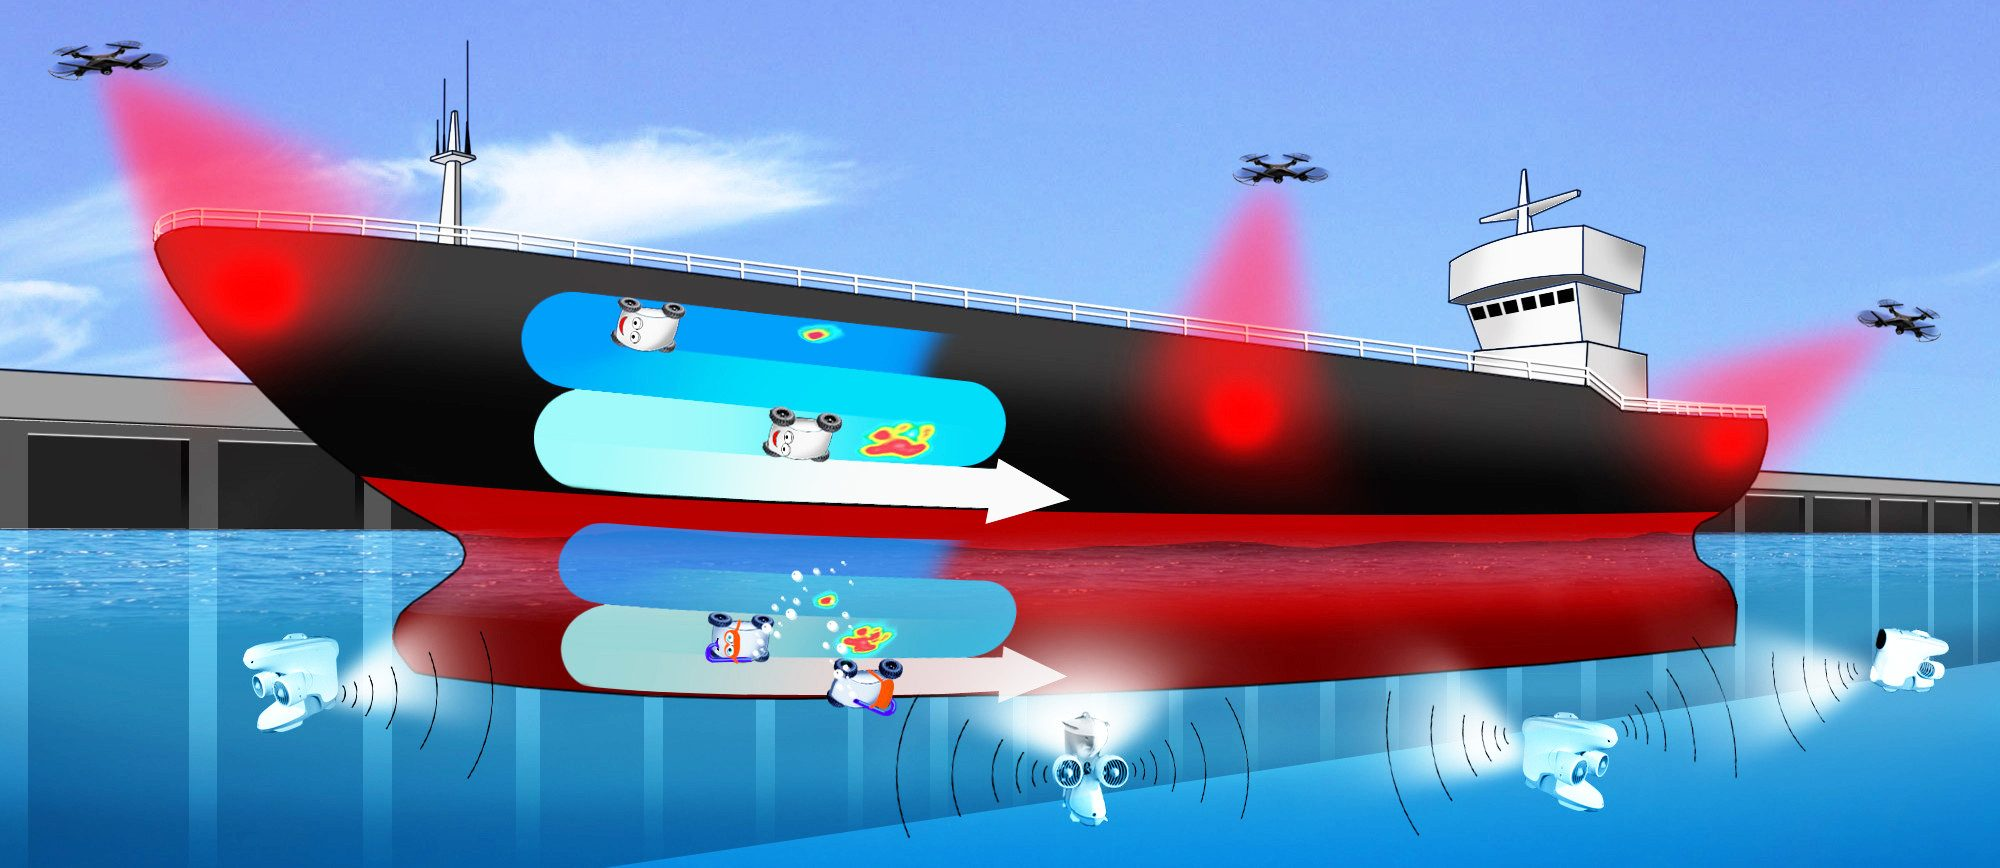
\includegraphics[width=0.8\textwidth]{graphics/Concept-Cartoon-NJ3-e1582812224528.jpg}
				\end{itemize}
			\end{frame}
		\subsection*{Définition du problème}
			\begin{frame}
				\frametitle{Introduction}
				\framesubtitle{Définition du problème}
				\begin{itemize}
					\item Inspection de structures métalliques
					\item Tomographie de la zone à inspecter
					\item Localiser des points de corrosion
					\item Ondes acoustiques (UGW)
				\end{itemize}
				\begin{block}{Problématique}
					Définir des stratégies de navigation multi-robots pour optimiser l'acquisition de données permettant de réaliser la tomographie des structures métalliques.
				\end{block}
			\end{frame}
		\subsection*{Aperçu des contributions}
			\begin{frame}
				\frametitle{Introduction}
				\framesubtitle{Aperçu des contributions}
				\begin{itemize}
					\item Développement de stratégies de navigation multi-robots pour l'inspection acoustique de structures métalliques
					\item Optimisation de l'acquisition de données pour la réalisation de la tomographie
					\item Résolution des problèmes de coordination et de synchronisation entre les robots
					\item Implémentation des méthodes de navigation dans un environnement de simulation
				\end{itemize}
			\end{frame}
	\section{Étude bibliographique et état de l'art}
		\begin{frame}
			\frametitle{Étude bibliographique et état de l'art}
			\tiny
			\nocite{9811581, HUTHWAITE2013979, s22093235, article455556, 9568841, 7487624, 7139673}
			\bibliographystyle{unsrt}
			\bibliography{RapportPFE}
		\end{frame}
	\section{Propositions scientifiques et techniques}
		\subsection{Définitions préliminaires}
			\begin{frame}[shrink=5]
				\frametitle{Propositions scientifiques et techniques}
				\framesubtitle{Définitions préliminaires}
				\begin{block}{Hypothèses}
					\begin{itemize}
						\item Environnement :
						\begin{itemize}
							\item espace 2D, borné et de taille connue
							\item obstacles localisés
							\item zones de corrosion non localisées
						\end{itemize}
						\item Robots :
						\begin{itemize}
							\item robots à 2 roues
							\item pose $(x, y, \theta)$ connue
							\item coût de rotation $cr$ et coût de translation $ct$ connus
							\item Nombre de robots $\ge$ 2
						\end{itemize}
						\item Perception :
						\begin{itemize}
							\item Robot est émetteur ou récepteur
							\item Émission et réception omnidirectionnelle d'ondes ultrasoniques (\textit{UGW})
							\item Si puissance de signal altérée, alors détection
							\item Détection parfaite et en temps réel
							\item Distance maximale d'émission et de réception $d_{max}$
						\end{itemize}
					\end{itemize}
				\end{block}
			\end{frame}
			\begin{frame}
				\frametitle{Propositions scientifiques et techniques}
				\framesubtitle{Définitions préliminaires}
				Modélisation de l'environnement et des robots
				\begin{figure}[H]
					\centering
					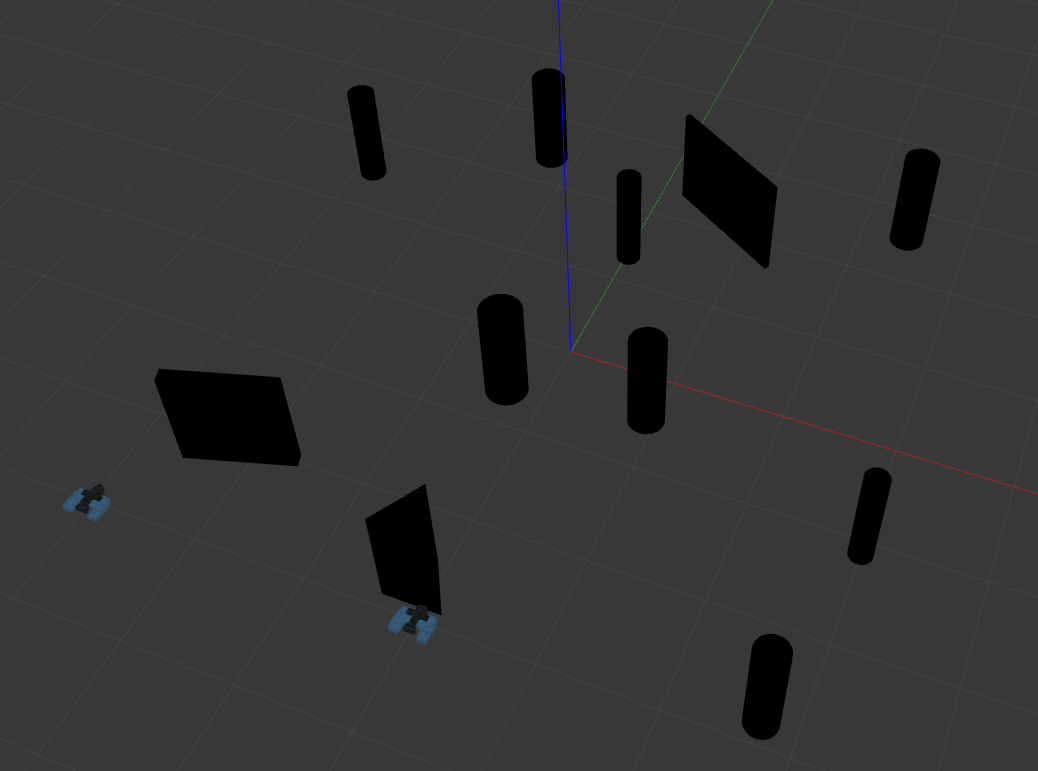
\includegraphics[width=0.7\linewidth]{graphics/exemple_model.png}
				\end{figure}
			\end{frame}
			\begin{frame}
				\frametitle{Propositions scientifiques et techniques}
				\framesubtitle{Définitions préliminaires}
				\begin{block}{Structure de données}
					\begin{itemize}
						\item Grille d'occupation :
						\begin{itemize}
							\item inconnu
							\item vide
							\item occupé
						\end{itemize}
					\end{itemize}
				\end{block}
				\begin{itemize}
					\item Enveloppes convexes des zones de corrosion
				\end{itemize}
			\end{frame}
		\subsection{Mise à jour de la grille d'occupation pour la cartographie}
			\begin{frame}
				\frametitle{Propositions scientifiques et techniques}
				\framesubtitle{Mise à jour de la grille d'occupation pour la cartographie}
				\begin{figure}
					\centering
					\begin{overprint}
						\onslide<1> 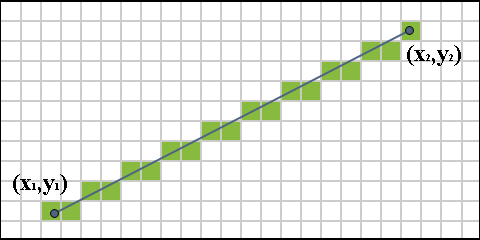
\includegraphics[width=0.95\linewidth]{graphics/Bresenham_line.png}
						\onslide<2> 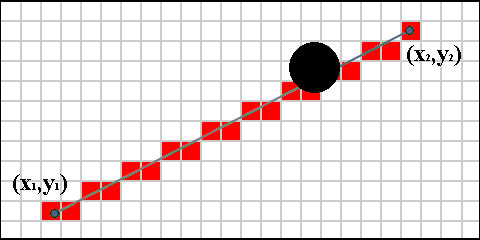
\includegraphics[width=0.95\linewidth]{graphics/Bresenham_line_2.png}
						\onslide<3> 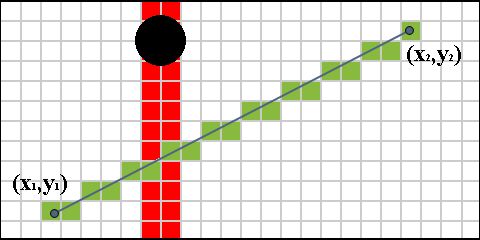
\includegraphics[width=0.95\linewidth]{graphics/Bresenham_line_3.png}
						\onslide<4> 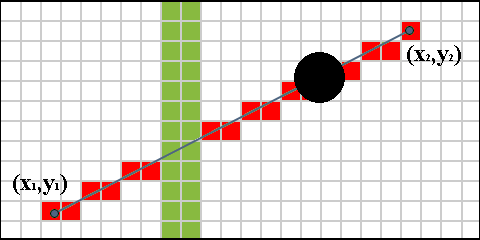
\includegraphics[width=0.95\linewidth]{graphics/Bresenham_line_4.png}
					\end{overprint}
				\end{figure}
				Algorithme de Bresenham \url{https://en.wikipedia.org/wiki/Bresenham\%27s_line_algorithm}
			\end{frame}
		\subsection{Stratégie de navigation \textit{peinture au rouleau}}
			\begin{frame}
				\frametitle{Propositions scientifiques et techniques}
				\framesubtitle{Stratégie de navigation \textit{peinture au rouleau}}
				\vspace{-5pt}
				\tiny
				\begin{block}{Description}
					\begin{itemize}\compresslist
						\item Nombre de robots $n \ge 2$, séparés par une distance $d < d_{max}$
						\item Chaque robot se déplace en ligne droite
						\item Les robots suivent une trajectoire parallèle
						\item Les robots se déplacent de manière \textbf{simultanée}
						\item Les robots se synchronisent régulièrement
					\end{itemize}
				\end{block}
				\vspace{-5pt}
				\begin{figure}
					\centering
					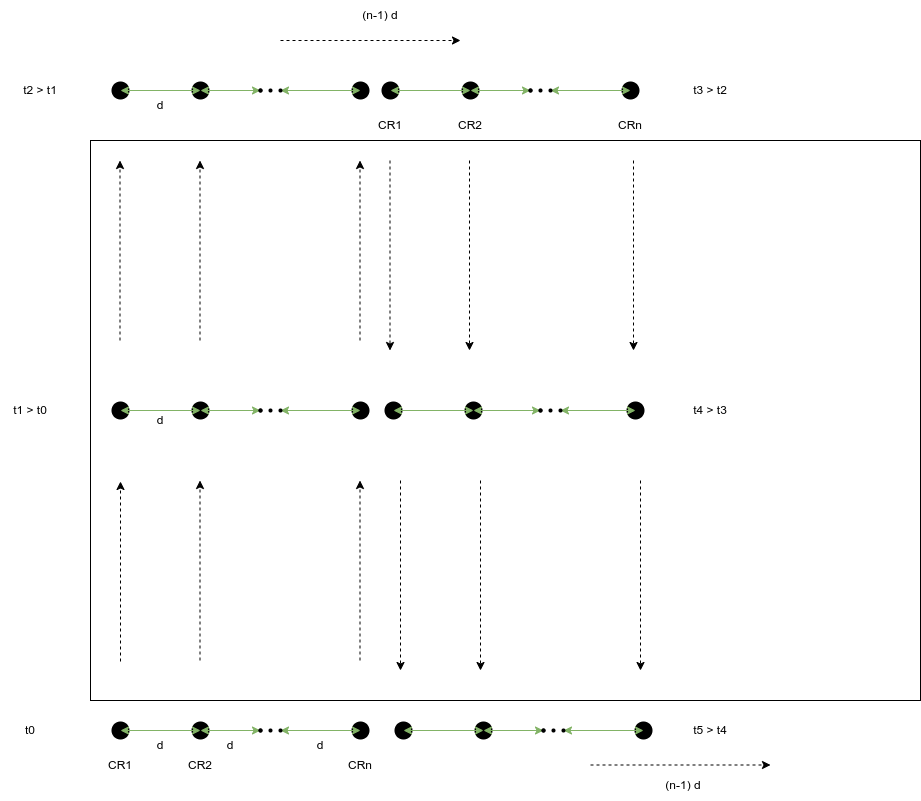
\includegraphics[width=0.5\linewidth]{graphics/peinture_au_rouleau.png}
				\end{figure}
			\end{frame}
			\begin{frame}
				\frametitle{Propositions scientifiques et techniques}
				\framesubtitle{Stratégie de navigation \textit{peinture au rouleau}}
				\begin{figure}[H]
					\centering
					\movie[label=show1, poster, showcontrols]{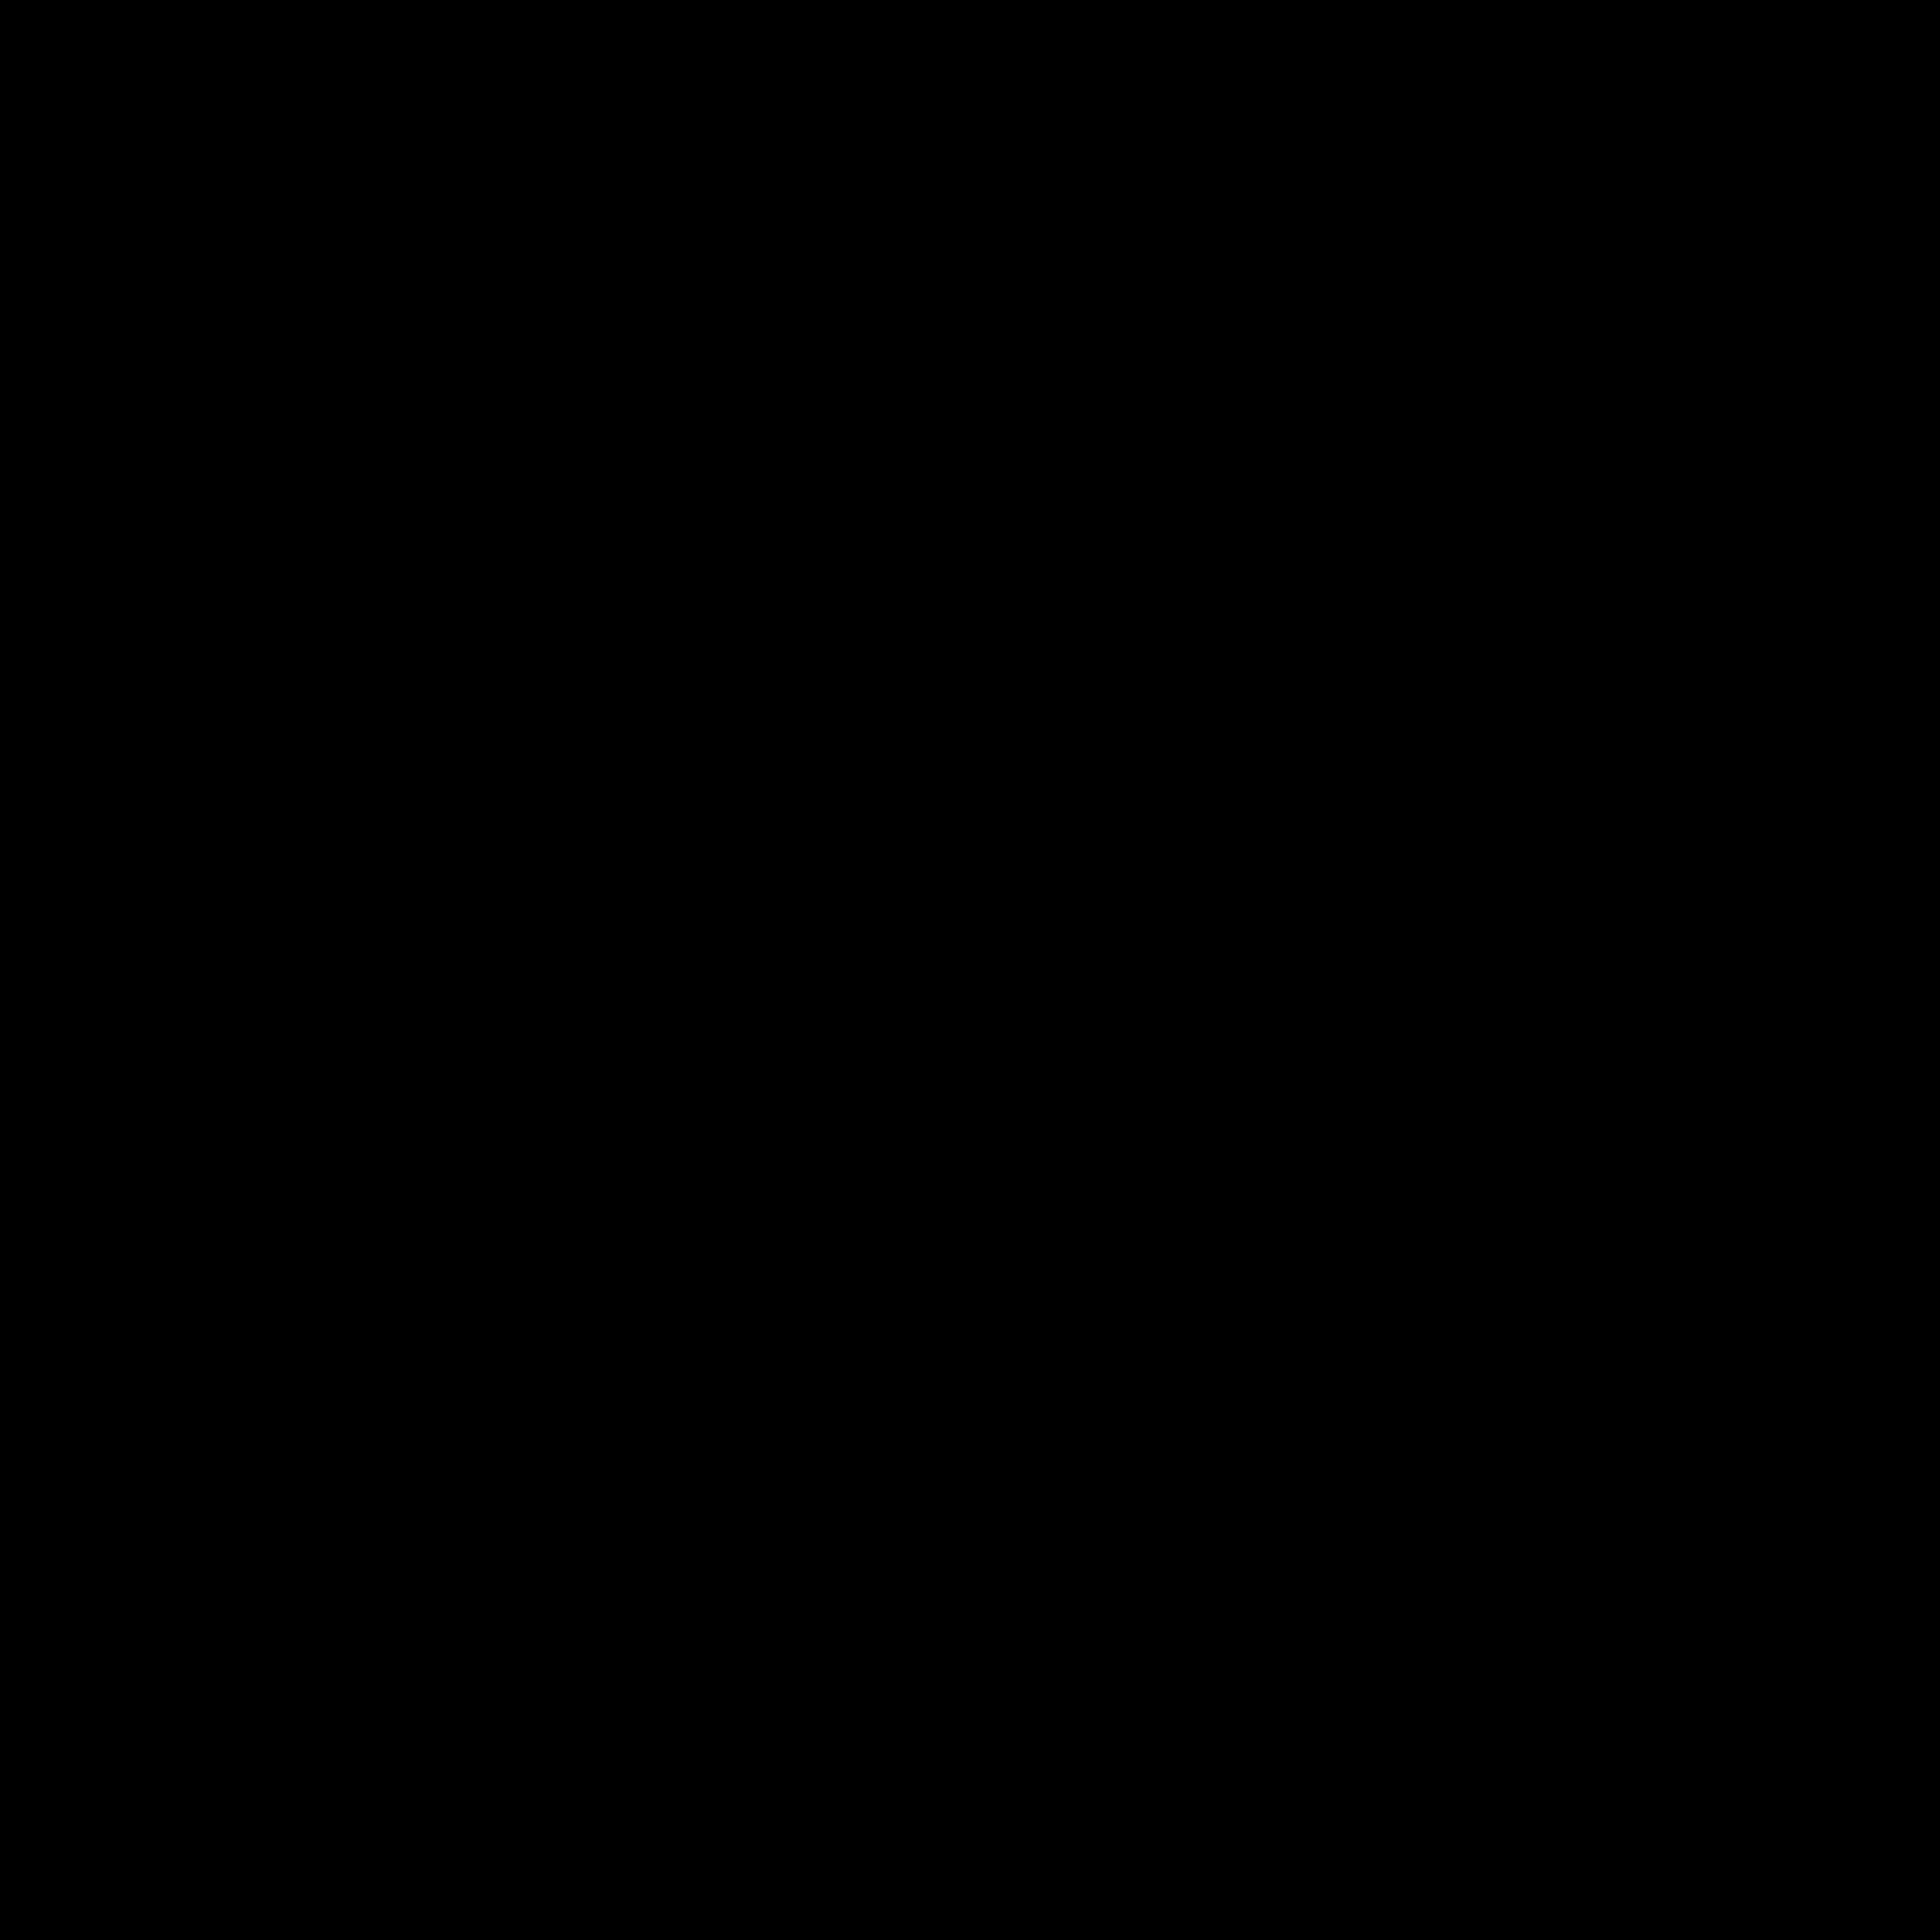
\includegraphics[scale=0.1]{graphics/black.png}}{graphics/peinture_au_rouleau.mp4}
				\end{figure}
			\end{frame}
			\begin{frame}
				\frametitle{Propositions scientifiques et techniques}
				\framesubtitle{Stratégie de navigation \textit{peinture au rouleau}}
				Cartographie résultante
				\begin{figure}
					\centering
					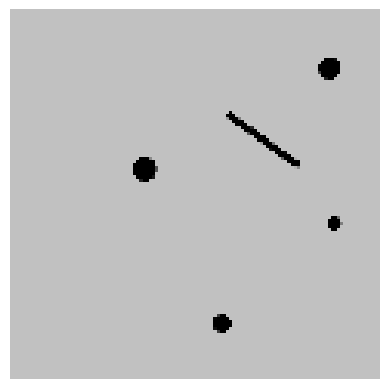
\includegraphics[width=0.3\linewidth]{graphics/test_05_flip.png}
					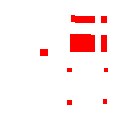
\includegraphics[width=0.3\linewidth]{graphics/occupancy_grid_example_par.png}
					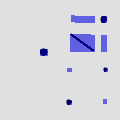
\includegraphics[width=0.3\linewidth]{graphics/both_example_par.png}
				\end{figure}
				score = 0.29

				temps = 4 m 20 s
			\end{frame}
			\begin{frame}
				\frametitle{Propositions scientifiques et techniques}
				\framesubtitle{Stratégie de navigation \textit{peinture au rouleau}}
				Implémentation
				\begin{itemize}
					\item Langage de programmation \textit{Python}, \textit{C++},
					\item Bibliothèques \textit{ROS}, \textit{OpenCV},
					\item Outil de simulation \textit{Gazebo},
					\item Outil de visualisation \textit{Rviz},
					\item Framework \textit{ROS Task Manager},
					\item Plugin UWB de l'équipe CHROMA.
				\end{itemize}
			\end{frame}
			\begin{frame}
				\frametitle{Propositions scientifiques et techniques}
				\framesubtitle{Stratégie de navigation \textit{peinture au rouleau}}
				\begin{exampleblock}{Avantages}
					\begin{itemize}
						\item Rapide.
					\end{itemize}
				\end{exampleblock}
				\begin{alertblock}{Inconvénients}
					\begin{itemize}
						\item Approximation des enveloppes peu précises,
						\item Zones fantômes.
					\end{itemize}
				\end{alertblock}
			\end{frame}
		\subsection{Stratégie de navigation \textit{ski nordique}}
			\begin{frame}
				\frametitle{Propositions scientifiques et techniques}
				\framesubtitle{Stratégie de navigation \textit{ski nordique}}
				\vspace{-5pt}
				\tiny
				\begin{block}{Description}
				\begin{itemize}\compresslist
						\item Nombre de robots $n \ge 2$, séparés par une distance $d < d_{max}$,
						\item Chaque robot se déplace en ligne droite,
						\item Les robots suivent une trajectoire parallèle,
						\item Les robots se déplacent de manière \textbf{alternée},
						\item Les robots se synchronisent régulièrement.
					\end{itemize}
				\end{block}
				\vspace{-5pt}
				\begin{figure}
					\centering
					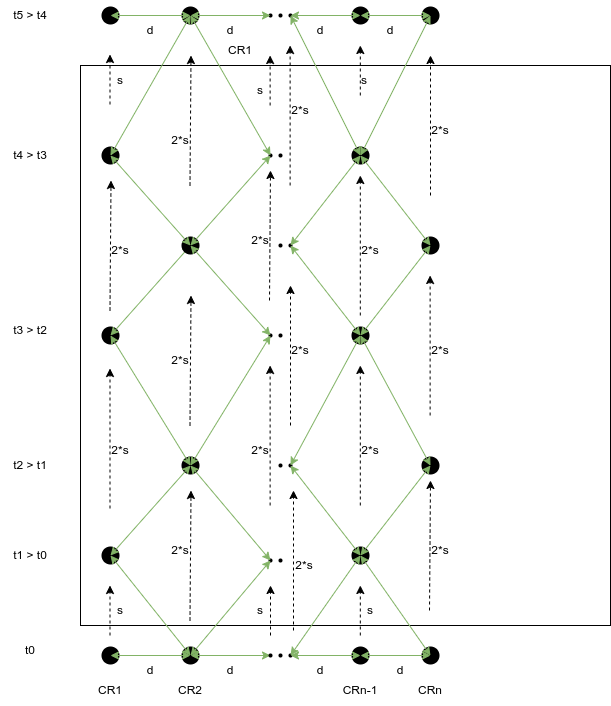
\includegraphics[width=0.35\linewidth]{graphics/ski_nordique_1.png}
					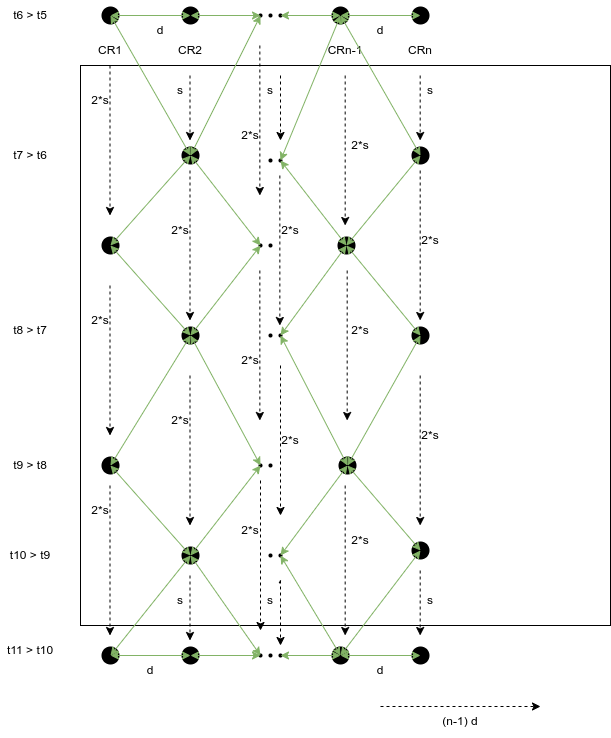
\includegraphics[width=0.35\linewidth]{graphics/ski_nordique_2.png}
				\end{figure}
			\end{frame}
			\begin{frame}
				\frametitle{Propositions scientifiques et techniques}
				\framesubtitle{Stratégie de navigation \textit{ski nordique}}
				\begin{figure}[H]
					\centering
					\movie[label=show1, poster, showcontrols]{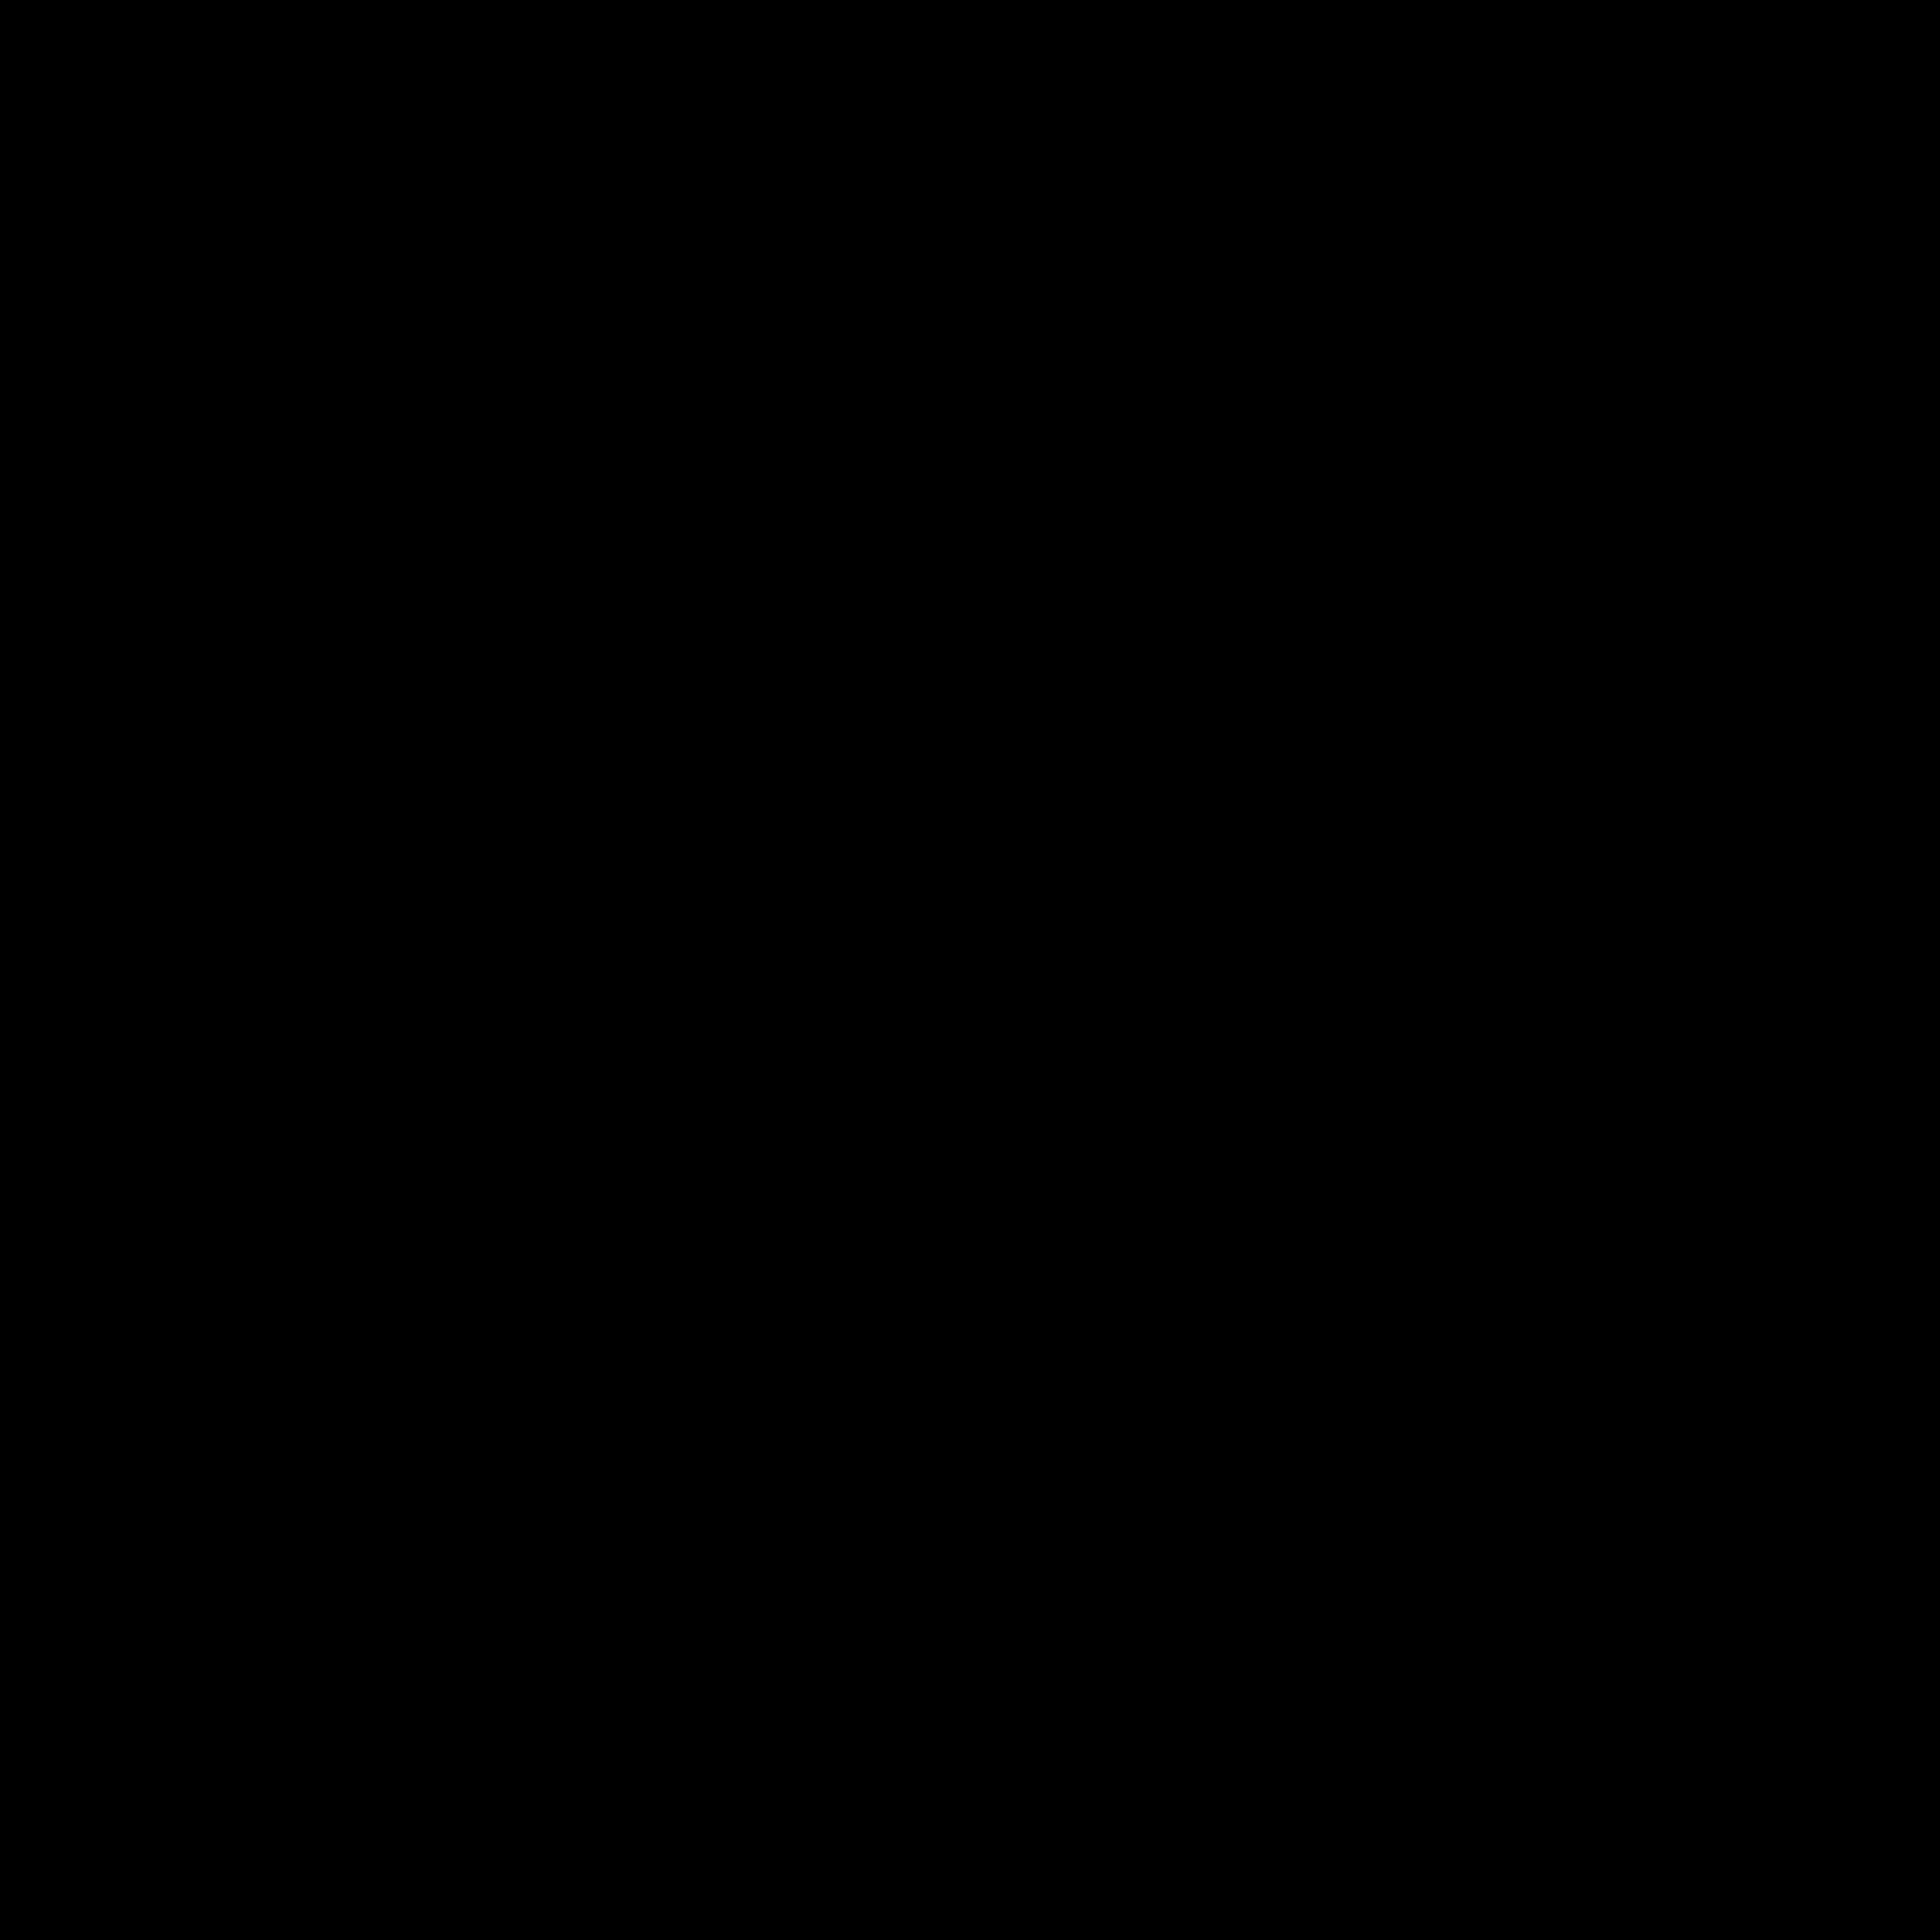
\includegraphics[scale=0.1]{graphics/black.png}}{graphics/ski_nordique_2.mp4}
				\end{figure}
			\end{frame}
			\begin{frame}
				\frametitle{Propositions scientifiques et techniques}
				\framesubtitle{Stratégie de navigation \textit{ski nordique}}
				Cartographie résultante
				\begin{figure}
					\centering
					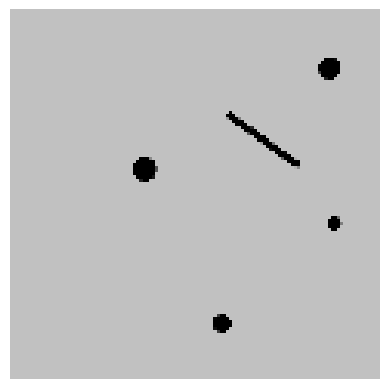
\includegraphics[width=0.3\linewidth]{graphics/test_05_flip.png}
					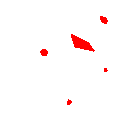
\includegraphics[width=0.3\linewidth]{graphics/occupancy_grid_example_sn.png}
					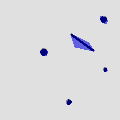
\includegraphics[width=0.3\linewidth]{graphics/both_example_sn.png}
				\end{figure}
				score = 0.63

				temps = 16 m 31 s
			\end{frame}
			\begin{frame}
				\frametitle{Propositions scientifiques et techniques}
				\framesubtitle{Stratégie de navigation \textit{ski nordique}}
				\begin{exampleblock}{Avantages (comparés à \textit{peinture au rouleau})}
					\begin{itemize}
						\item Approximation des enveloppes plus précises,
					\end{itemize}
				\end{exampleblock}
				\begin{alertblock}{Inconvénients comparés à peinture au rouleau}
					\begin{itemize}
						\item Plus lent,
						\item Zones fantômes.
					\end{itemize}
				\end{alertblock}
			\end{frame}
		\subsection{Stratégie de navigation \textit{investigation polygonale}}
			\begin{frame}
				\frametitle{Propositions scientifiques et techniques}
				\framesubtitle{Stratégie de navigation \textit{investigation polygonale}}
				\vspace{-5pt}
				\tiny
				\begin{block}{Description}\compresslist
					\begin{itemize}
						\item Utilise la cartographie résultante d'une des deux stratégies précédentes,
						\item $k \ge 1$ équipes de $n \ge 2$ robots,
						\item Les robots d'une même équipe se placent sur des sommets consécutifs d'un polygone convexe $P$ à $p$ sommets,
						\item Les robots se déplacent, les uns après les autres, en suivant le chemin défini par le périmètre du polygone $P$.
						\item L'algorithme se termine lorsque les sommets initialement occupés par les robots sont à nouveau occupés.
					\end{itemize}
				\end{block}
				\vspace{-5pt}
				\begin{figure}
					\centering
					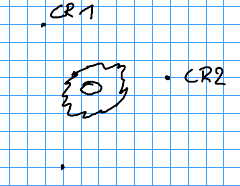
\includegraphics[height=0.2\linewidth]{graphics/triangle_1.png}
					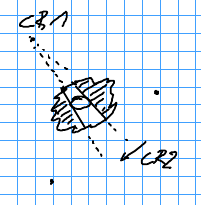
\includegraphics[height=0.2\linewidth]{graphics/triangle_2.png}
					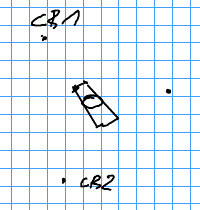
\includegraphics[height=0.2\linewidth]{graphics/triangle_3.png}
					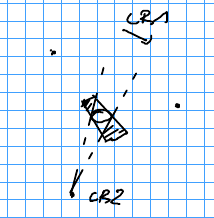
\includegraphics[height=0.2\linewidth]{graphics/triangle_4.png}
					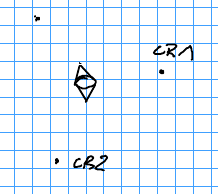
\includegraphics[height=0.2\linewidth]{graphics/triangle_5.png}
					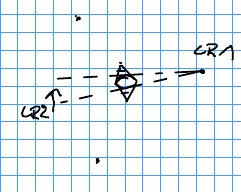
\includegraphics[height=0.2\linewidth]{graphics/triangle_6.png}
					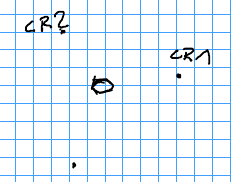
\includegraphics[height=0.2\linewidth]{graphics/triangle_7.png}
				\end{figure}
			\end{frame}
			\begin{frame}
				\frametitle{Propositions scientifiques et techniques}
				\framesubtitle{Stratégie de navigation \textit{investigation polygonale}}
				\begin{figure}[H]
					\centering
					\movie[label=show1, poster, showcontrols]{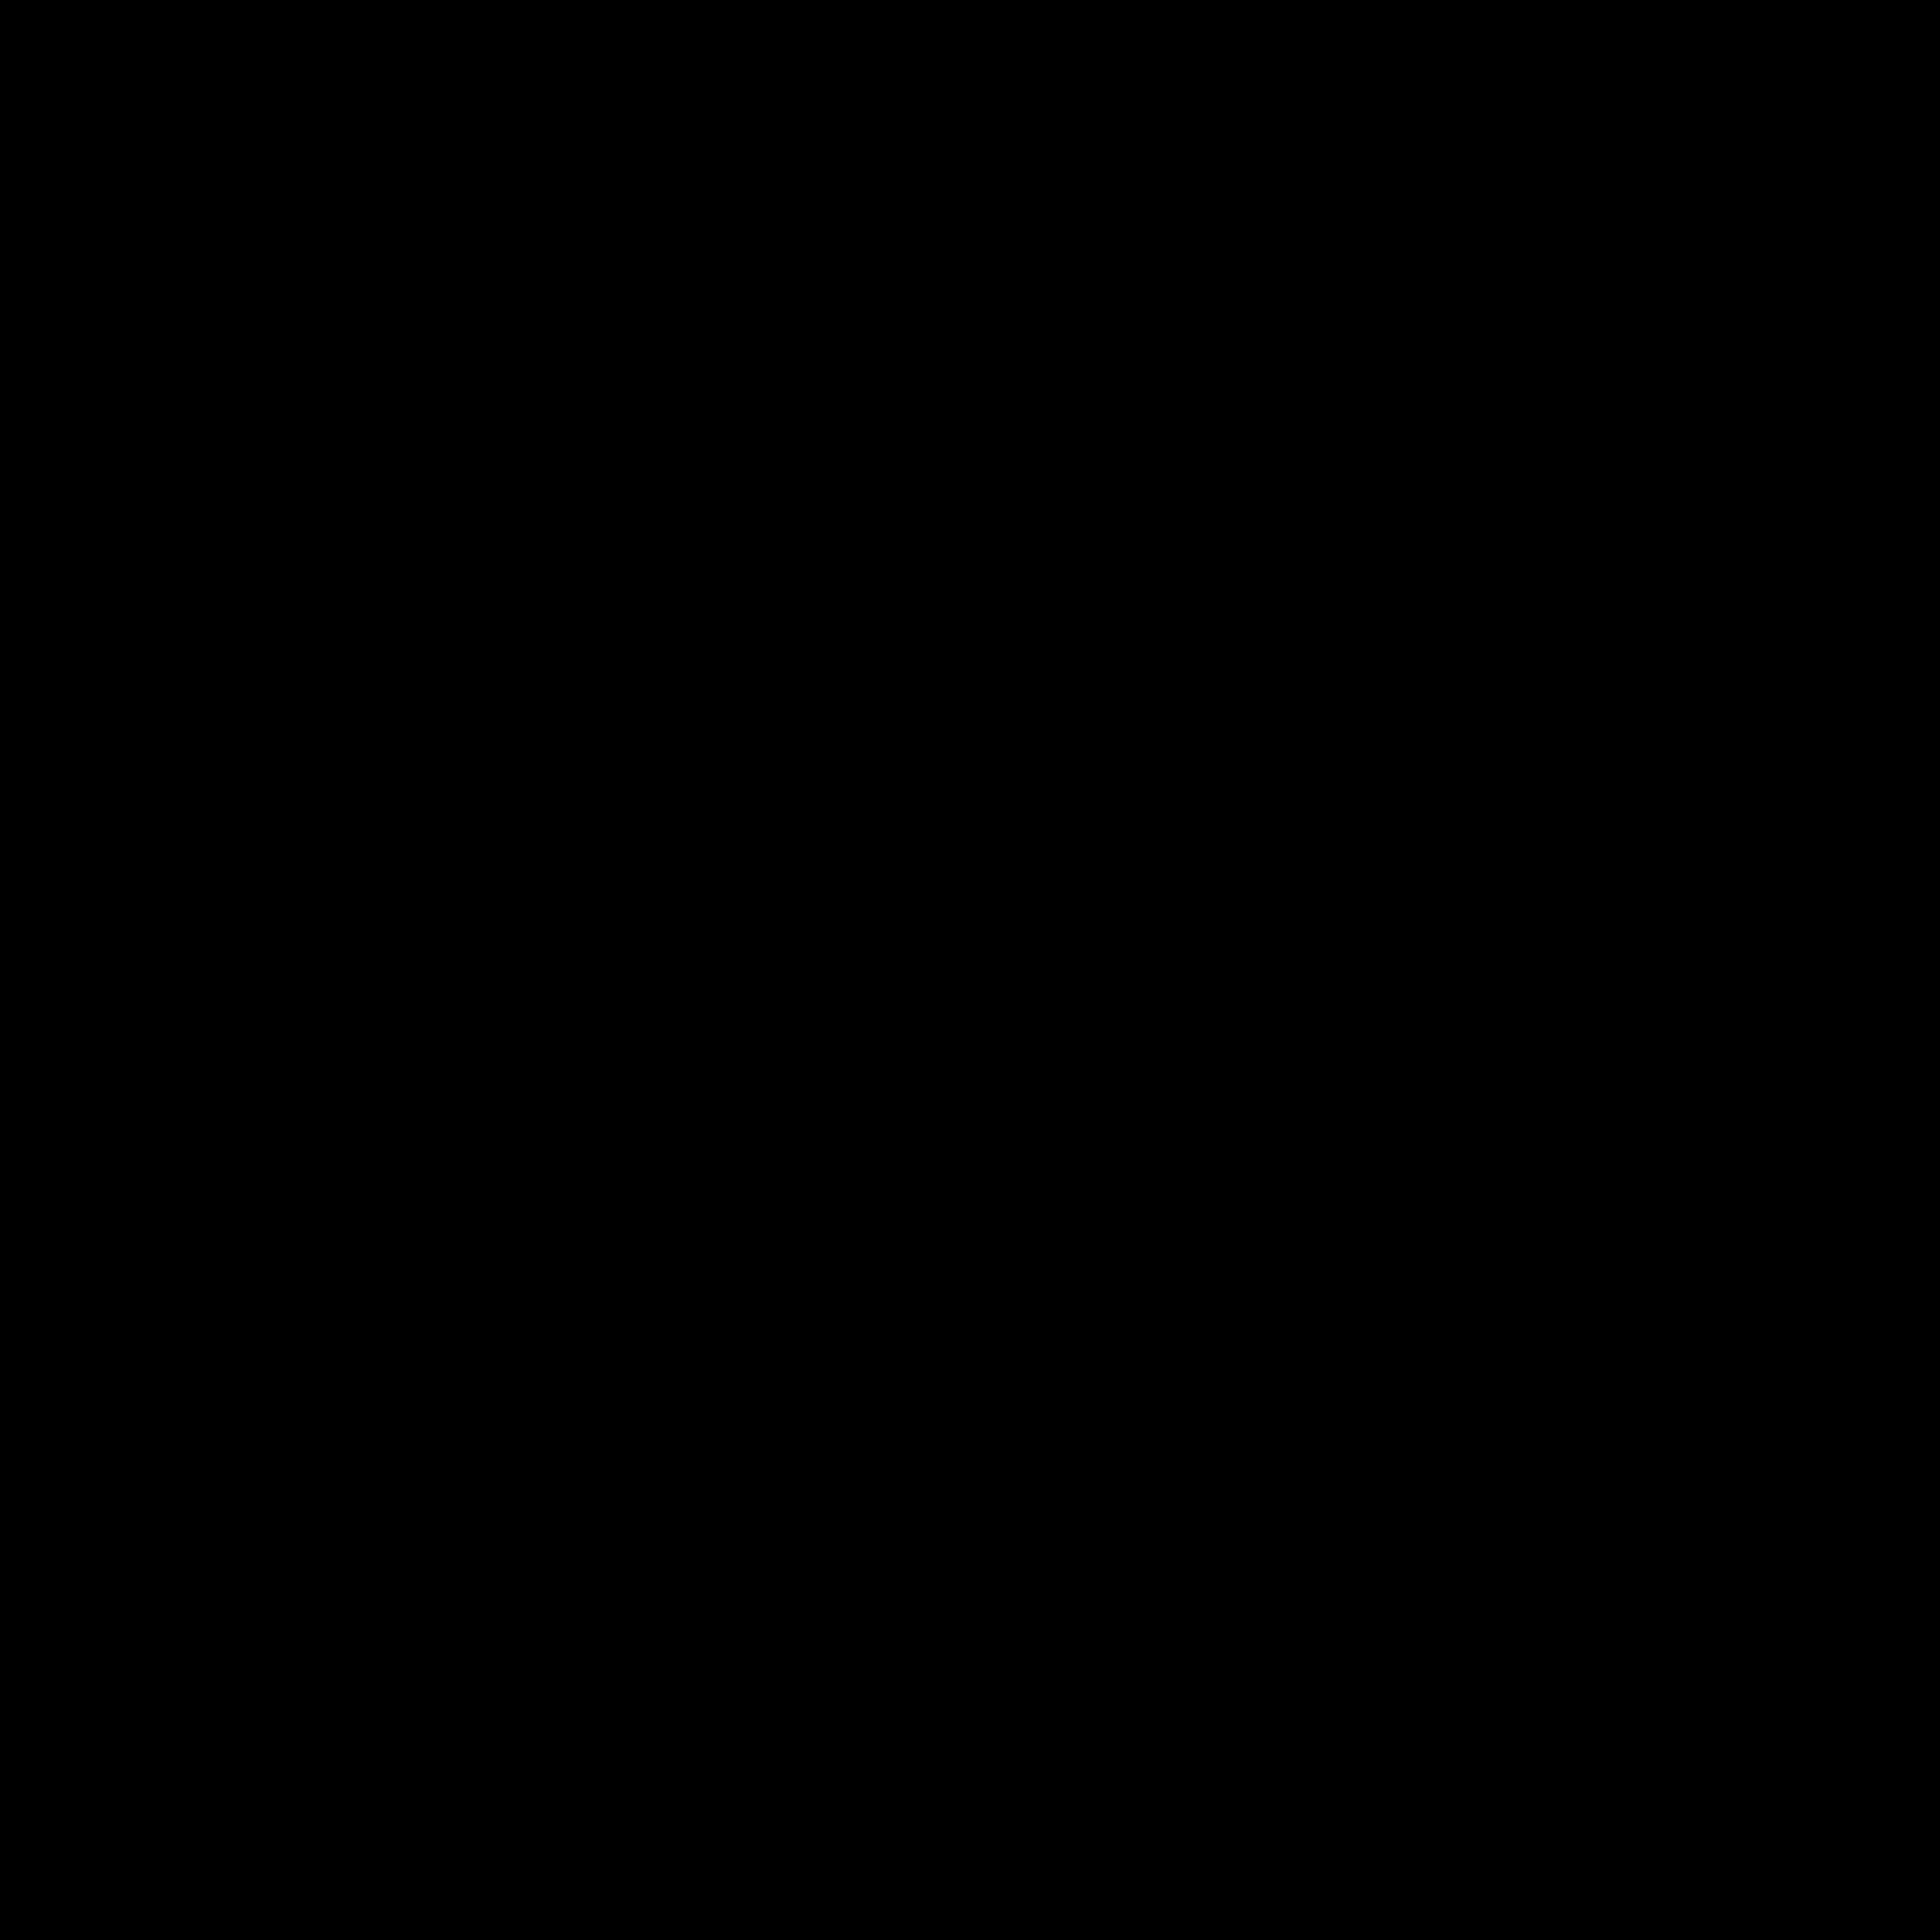
\includegraphics[scale=0.1]{graphics/black.png}}{graphics/investigation_polygonale.mp4}
				\end{figure}
			\end{frame}
			\begin{frame}
				\frametitle{Propositions scientifiques et techniques}
				\framesubtitle{Stratégie de navigation \textit{investigation polygonale}}
				Cartographie résultante
				\begin{figure}
					\centering
					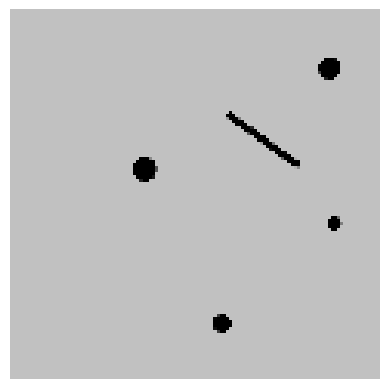
\includegraphics[width=0.3\linewidth]{graphics/test_05_flip.png}
					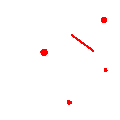
\includegraphics[width=0.3\linewidth]{graphics/occupancy_grid_example_ip.png}
					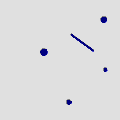
\includegraphics[width=0.3\linewidth]{graphics/both_example_ip.png}
				\end{figure}
				score = 0.86

				temps = 9 m 31 s (13 m 51 s)
			\end{frame}
			\begin{frame}
				\frametitle{Propositions scientifiques et techniques}
				\framesubtitle{Stratégie de navigation \textit{investigation polygonale}}
				\begin{enumerate}
					\item Extraction des zones de corrosion,
					\item Détermination de l'ordre d'investigation des zones de corrosion.
				\end{enumerate}
				\begin{block}{Extraction des zones de corrosion}
					\begin{itemize}
						\item Conversion de la grille d'occupation en graphe,
						\item Algorithme d'extraction de composantes fortement connexes,
					\end{itemize}
				\end{block}
				\begin{block}{Détermination de l'ordre d'investigation des zones de corrosion}
					\begin{itemize}
						\item Algorithme TSP ($k = 1$)
						\item Algorithme mTSP ($k > 1$)
					\end{itemize}
				\end{block}
			\end{frame}
			\begin{frame}
				\frametitle{Propositions scientifiques et techniques}
				\framesubtitle{Stratégie de navigation \textit{investigation polygonale}}
				Implémentation
				\begin{itemize}
					\item Bibliothèque \textit{OpenCV} pour l'extraction des zones de corrosion,
					\item Bibliothèque \textit{Gurobi} pour le TSP,
					\item MDMTSPV\_GA - Multiple Depot Multiple Traveling Salesmen Problem solved by Genetic Algorithm, Elad Kivelevitch, pour le mTSP.
				\end{itemize}
			\end{frame}
			\begin{frame}
				\frametitle{Propositions scientifiques et techniques}
				\framesubtitle{Stratégie de navigation \textit{investigation polygonale}}
				\begin{exampleblock}{Avantages}
					\begin{itemize}
						\item Approximation des enveloppes précise (proportionnellement au nombre de sommets du polygone)
						\item Permet de rapidement éliminer les zones fantômes.
					\end{itemize}
				\end{exampleblock}
				\begin{alertblock}{Inconvénients}
					\begin{itemize}
						\item Lent (proportionnellement au nombre de sommets du polygone, inversement proportionnel au nombre de robots, proportionnellement au nombre de zones de corrosion),
					\end{itemize}
				\end{alertblock}
			\end{frame}
	\section{Expérimentations, validations et évaluations}
		\subsection{Métrique d'évaluation}
			\begin{frame}
				\frametitle{Expérimentations, validations et évaluations}
				\framesubtitle{Métrique d'évaluation}
				\small
				\vspace{-5pt}
				Kappa de Cohen :
				\vspace{-5pt}
				\begin{equation*}
					\kappa = \frac{p_o - p_e}{1 - p_e}
				\end{equation*}
				\vspace{-5pt}
				avec :
				\begin{itemize}
					\item $p_o$ : précision observée,
					\item $p_e$ : précision aléatoire,
					\item $\kappa$ : mesure une classification binaire, en la comparant à une classification aléatoire.
				\end{itemize}
				\vspace{-15pt}
				\begin{table}
					\centering
					\begin{tabular}{|c|c|}
						\hline
						$\kappa$ & Interprétation \\
						\hline
						$< 0$ & Désaccord \\
						\hline
						$0.00 - 0.20$ & Accord très faible \\
						\hline
						$0.21 - 0.40$ & Accord faible \\
						\hline
						$0.41 - 0.60$ & Accord modéré \\
						\hline
						$0.61 - 0.80$ & Accord fort \\
						\hline
						$0.81 - 1.00$ & Accord presque parfait \\
						\hline
					\end{tabular}
				\end{table}
				Kappa de Cohen \url{https://en.wikipedia.org/wiki/Cohen\%27s_kappa}
			\end{frame}
		\subsection{Expérimentations}
			\begin{frame}
				\frametitle{Expérimentations, validations et évaluations}
				\framesubtitle{Expérimentations}
				\begin{table}[H]
					\centering
					\begin{tabular}{|c|c|c|}
						\hline
						Stratégie & Paramètre & Valeurs \\
						\hline
						\multirow{2}{*}{\textit{peinture au rouleau}} & $n$ & 2 \\
						& $d$ & 1, 2, 3, 6 (mètres) \\
						\hline
						\multirow{3}{*}{\textit{ski nordique}} & $n$ & 2 \\
						& $d$ & 1, 2, 3, 6 (mètres) \\
						& $s$ & 1, 2, 3, 6 (mètres) \\
						\hline
						\multirow{5}{*}{\textit{investigation polygonale}} & stratégie initiale & \textit{peinture au rouleau} \\
						& $d$ & 1, 2, 3, 6 (mètres) \\
						& $n$ & 2 \\
						& $k$ & 1 \\
						& $p$ & 4, 6 \\
						\hline
					\end{tabular}
				\end{table}
			\end{frame}
			\begin{frame}
				\frametitle{Expérimentations, validations et évaluations}
				\framesubtitle{Expérimentations}
				\begin{figure}[H]
					\centering
					\begin{columns}
						\begin{column}{0.14\textwidth}
							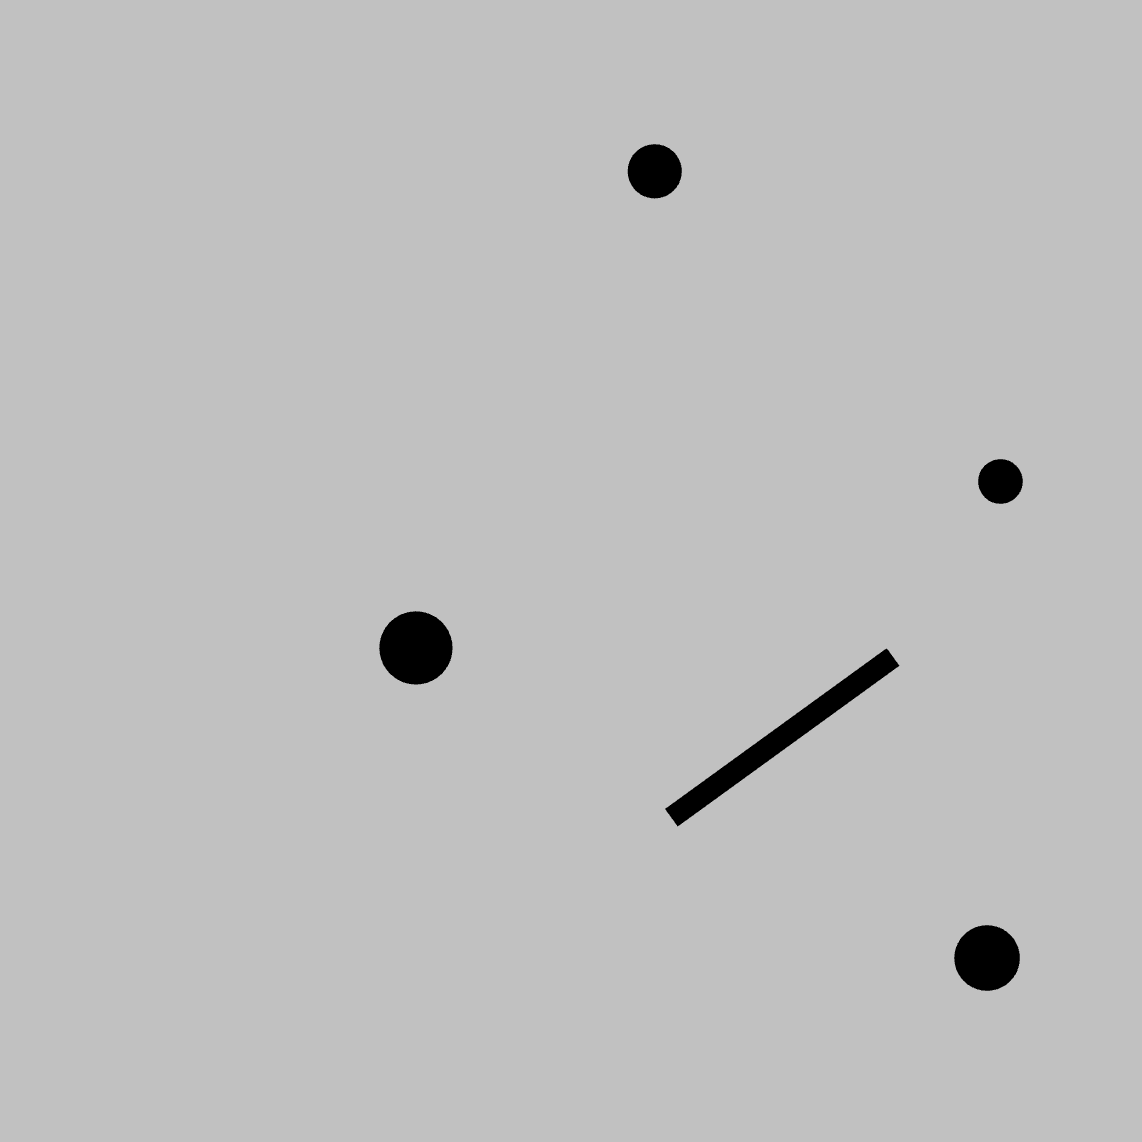
\includegraphics[width=1\linewidth]{graphics/test_model_05_1.png}
							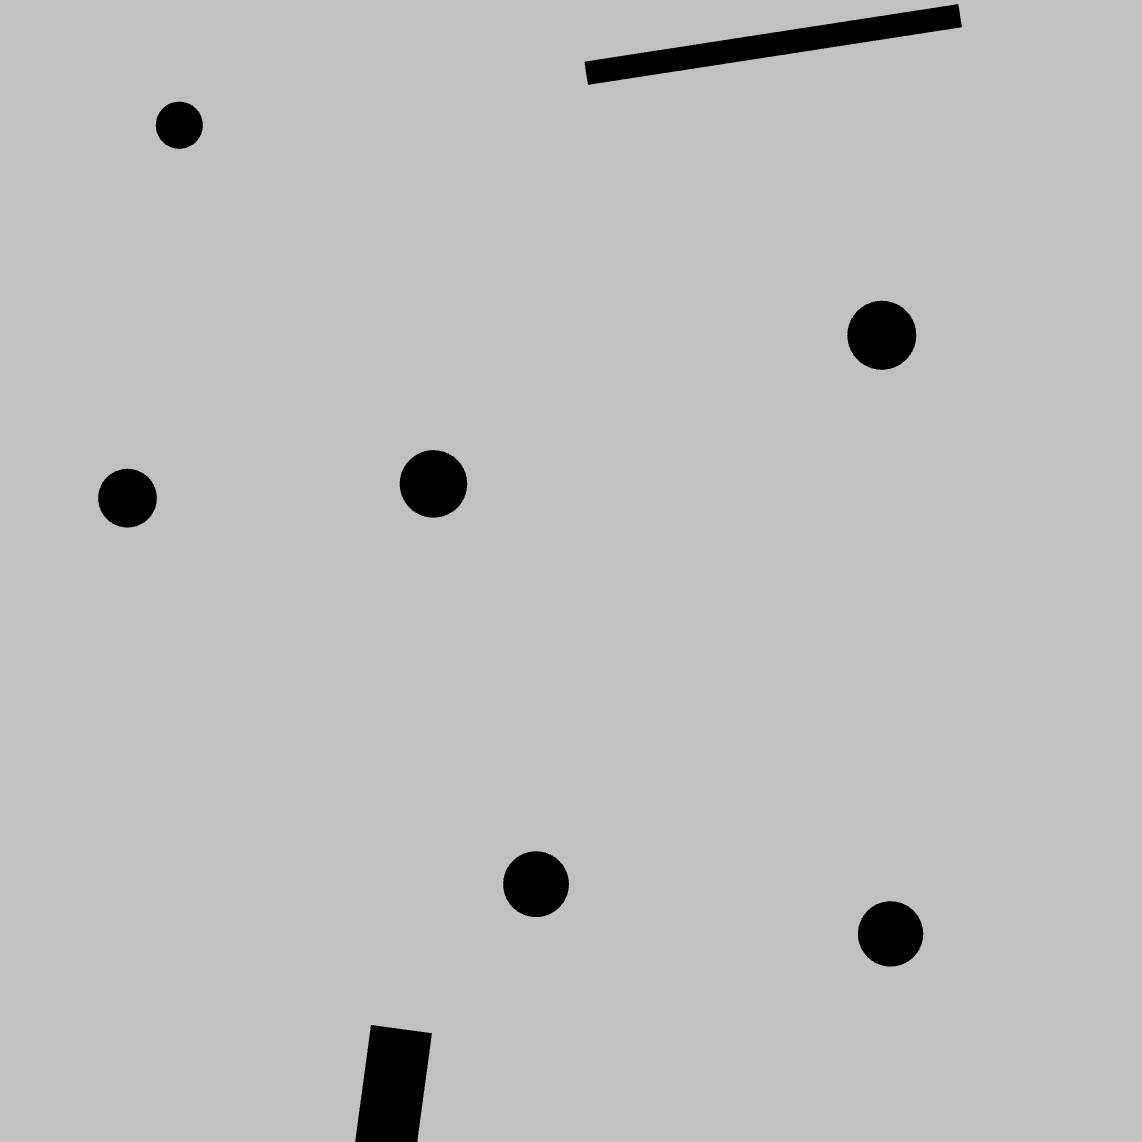
\includegraphics[width=1\linewidth]{graphics/test_model_08_1.png}
							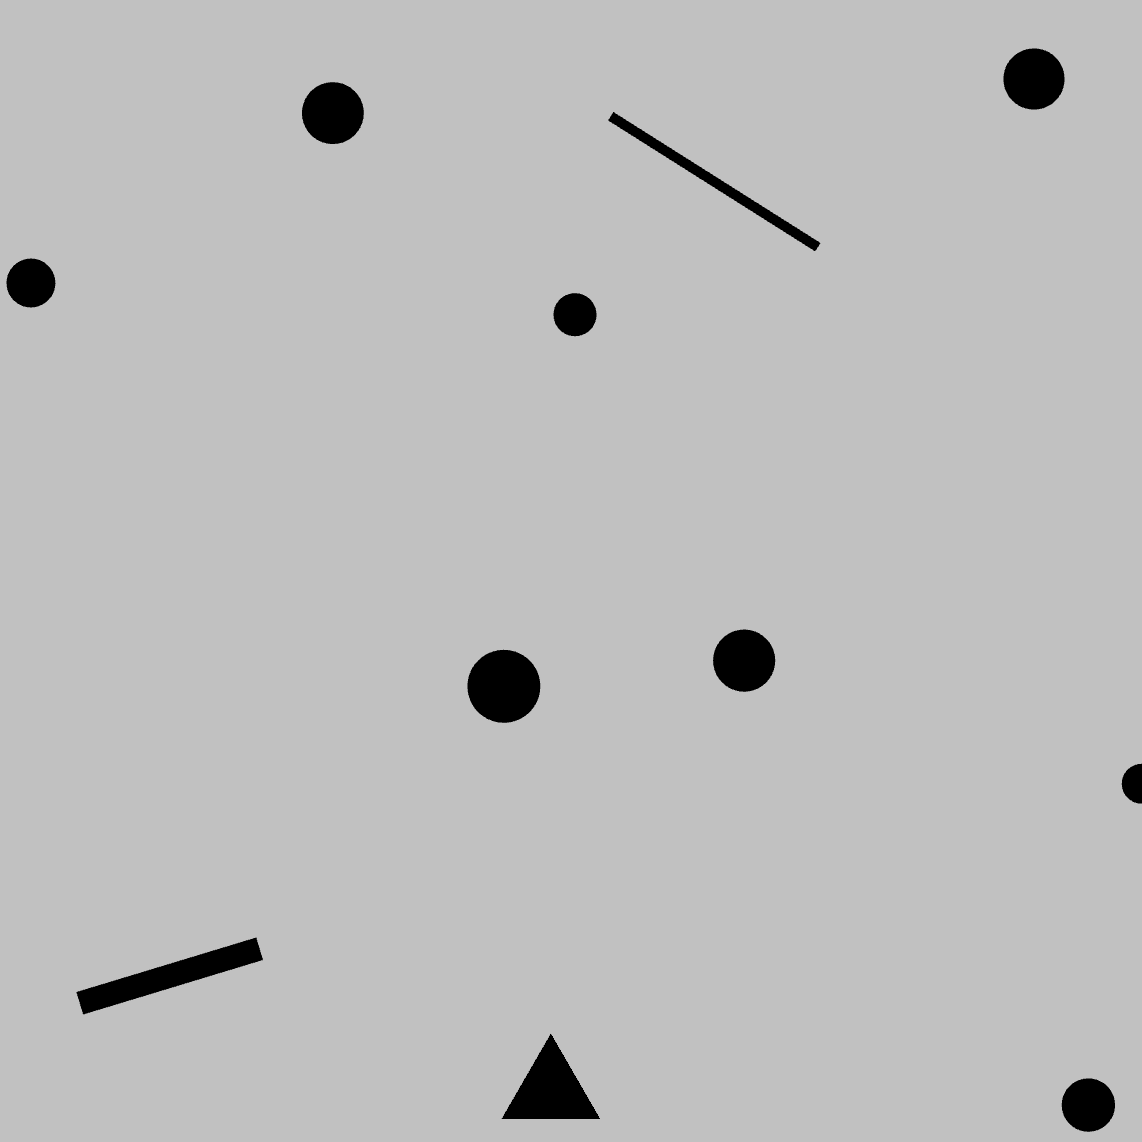
\includegraphics[width=1\linewidth]{graphics/test_model_11_1.png}
							
\includegraphics[width=1\linewidth]{graphics/test_model_15_1.png}
						\end{column}
						\begin{column}{0.14\textwidth}
							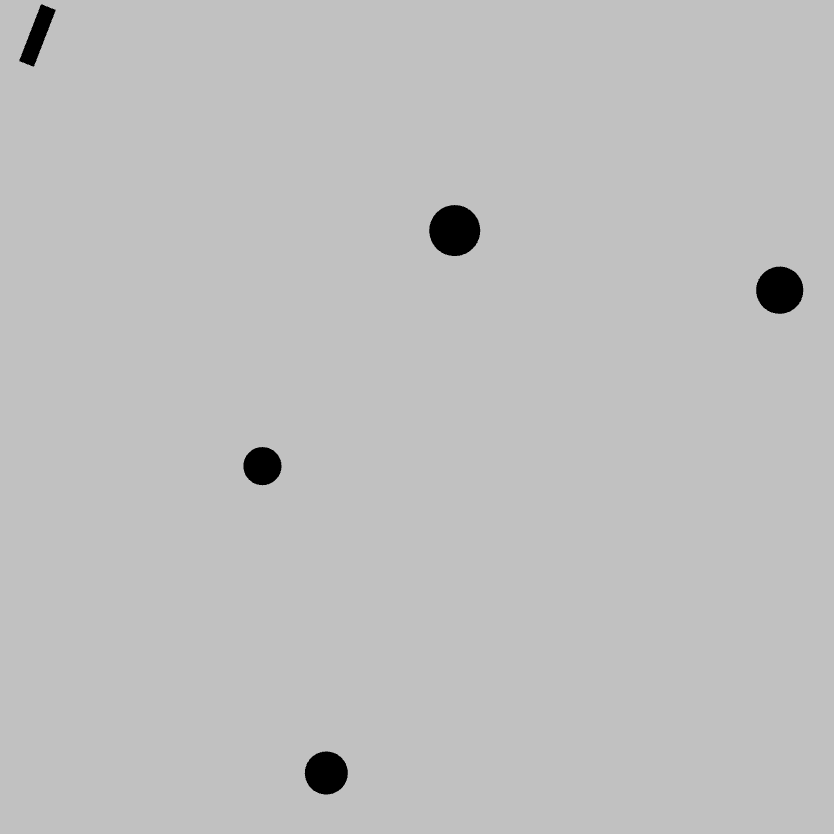
\includegraphics[width=1\linewidth]{graphics/test_model_05_2.png}
							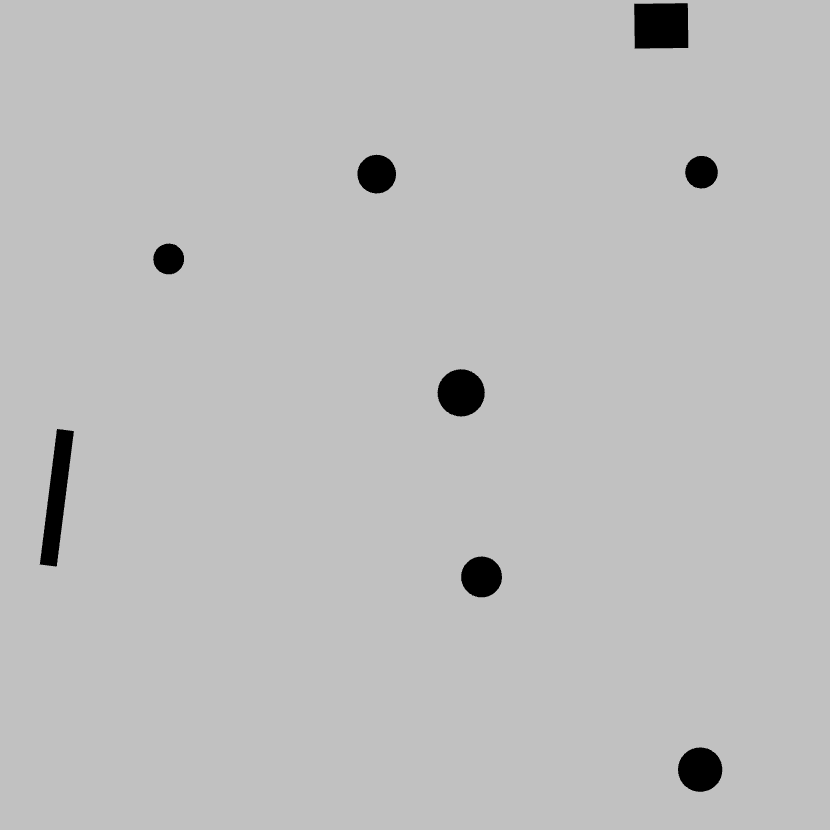
\includegraphics[width=1\linewidth]{graphics/test_model_08_2.png}
							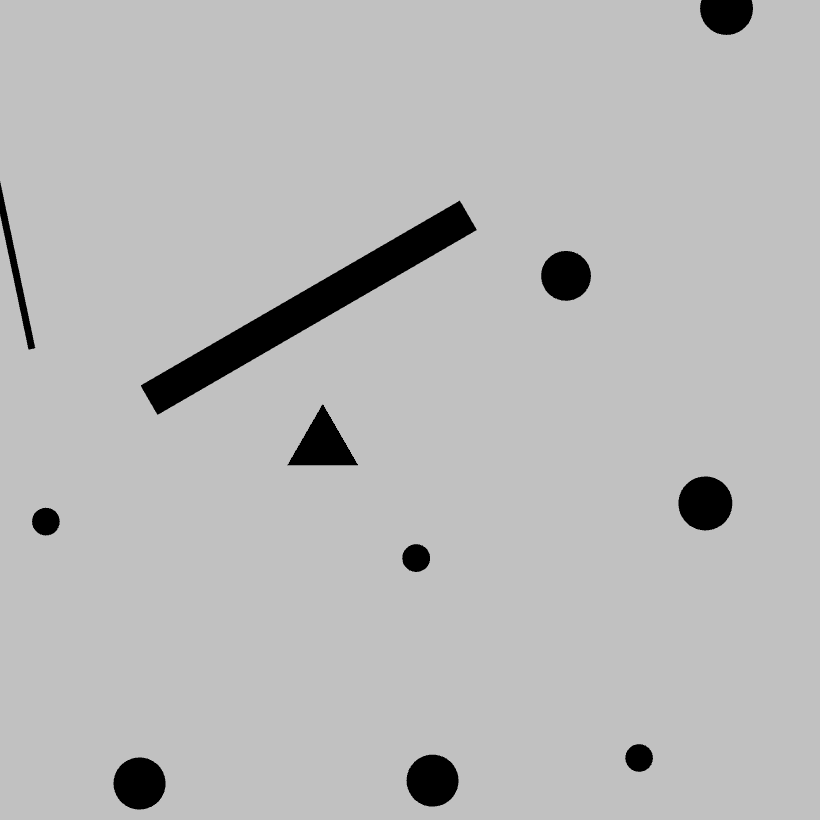
\includegraphics[width=1\linewidth]{graphics/test_model_11_2.png}
							
\includegraphics[width=1\linewidth]{graphics/test_model_15_2.png}
						\end{column}
						\begin{column}{0.14\textwidth}
							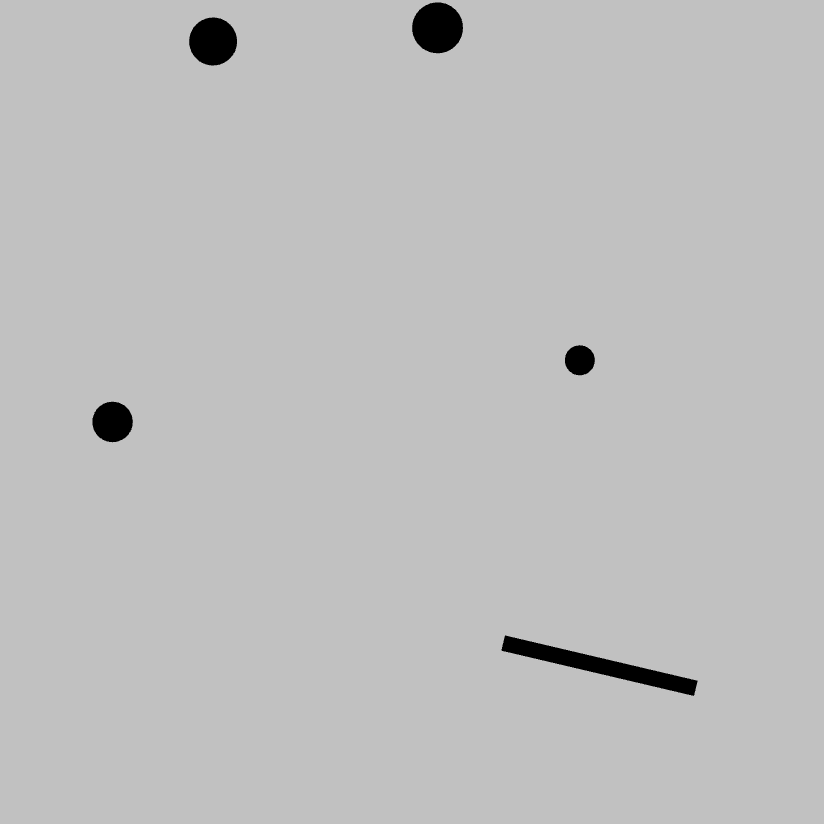
\includegraphics[width=1\linewidth]{graphics/test_model_05_3.png}
							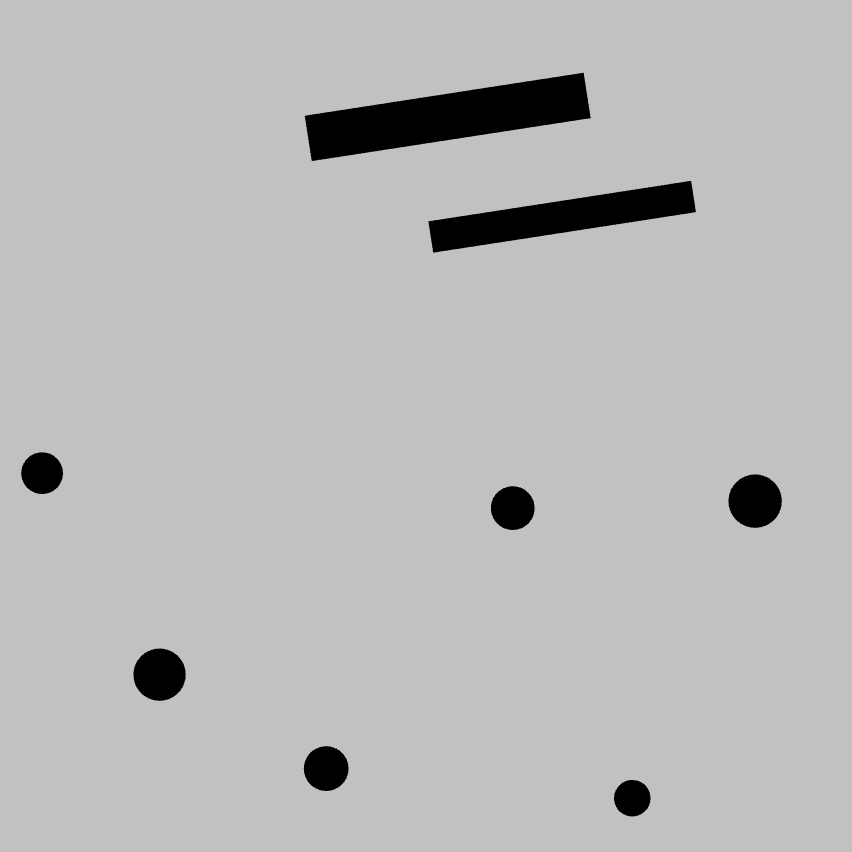
\includegraphics[width=1\linewidth]{graphics/test_model_08_3.png}
							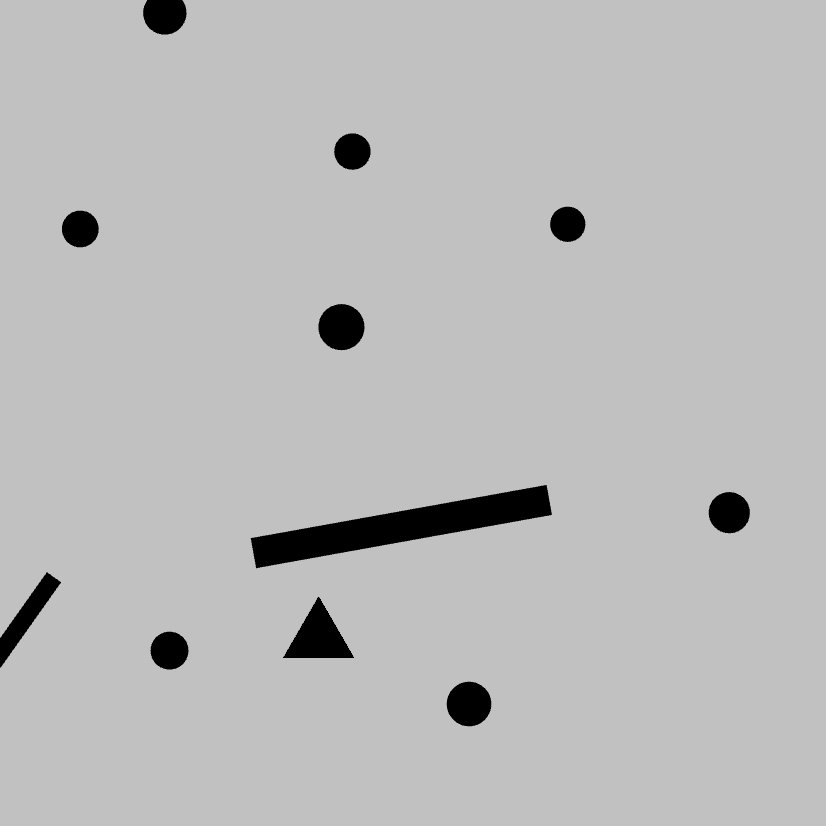
\includegraphics[width=1\linewidth]{graphics/test_model_11_3.png}
							
\includegraphics[width=1\linewidth]{graphics/test_model_15_3.png}
						\end{column}
						\begin{column}{0.14\textwidth}
							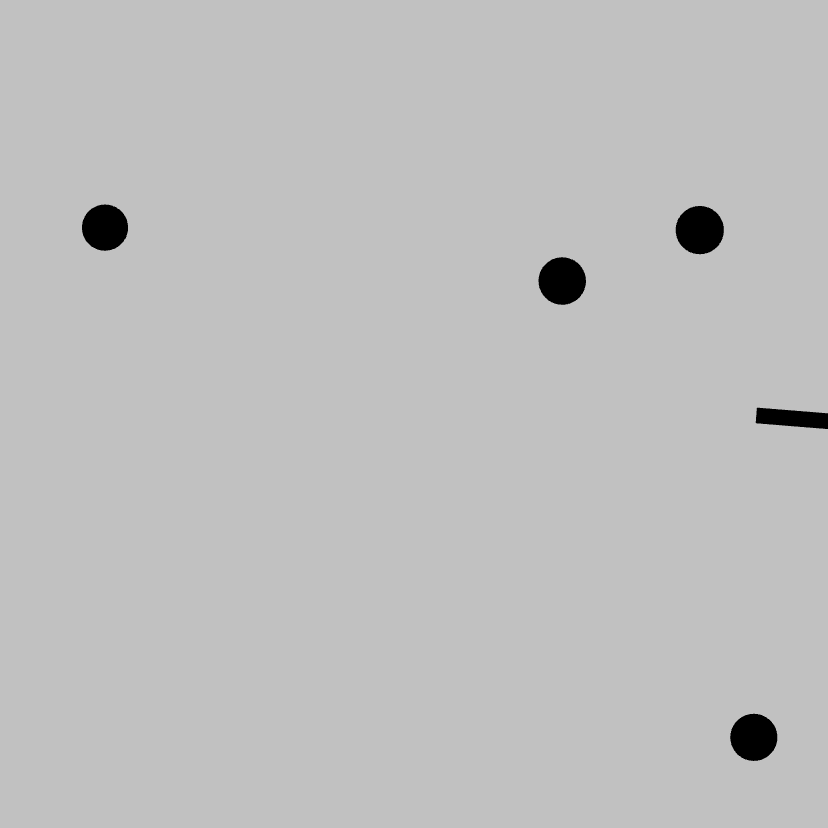
\includegraphics[width=1\linewidth]{graphics/test_model_05_4.png}
							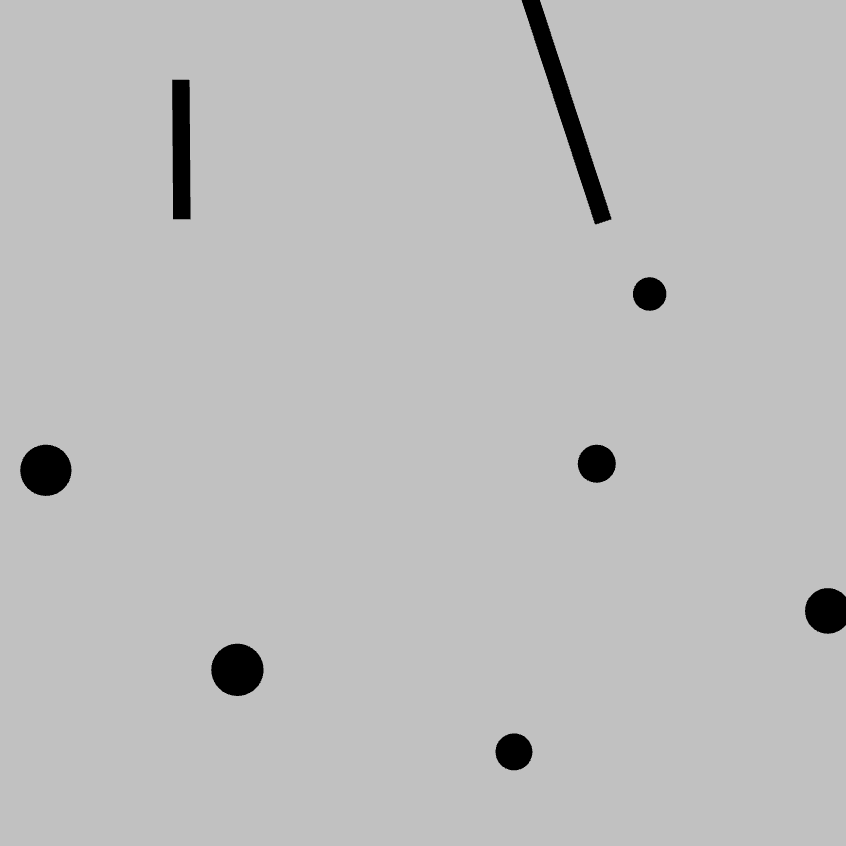
\includegraphics[width=1\linewidth]{graphics/test_model_08_4.png}
							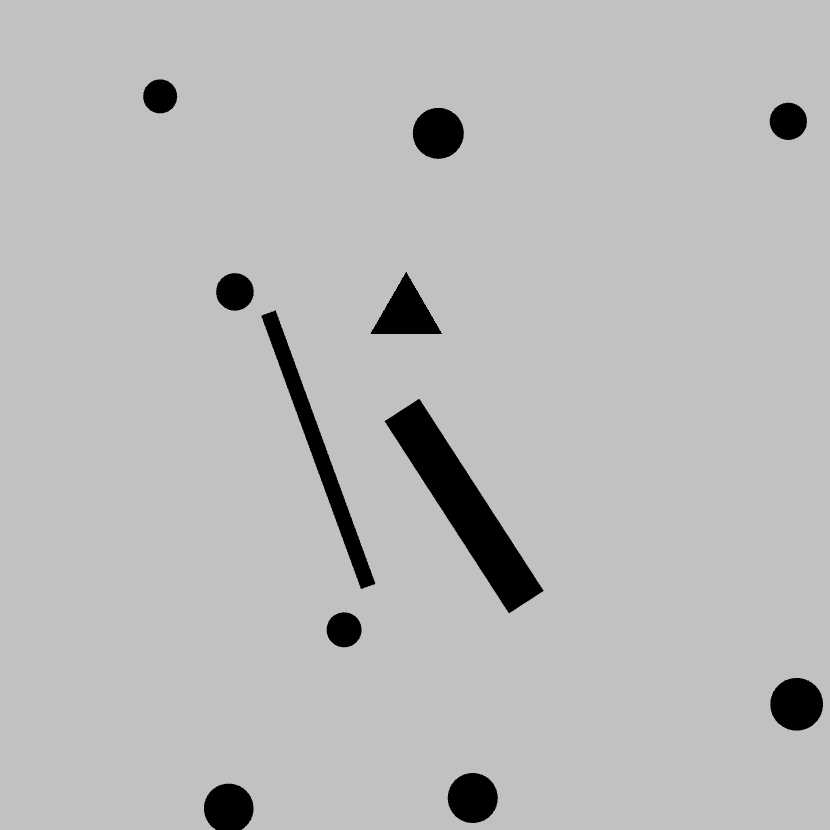
\includegraphics[width=1\linewidth]{graphics/test_model_11_4.png}
							
\includegraphics[width=1\linewidth]{graphics/test_model_15_4.png}
						\end{column}
						\begin{column}{0.14\textwidth}
							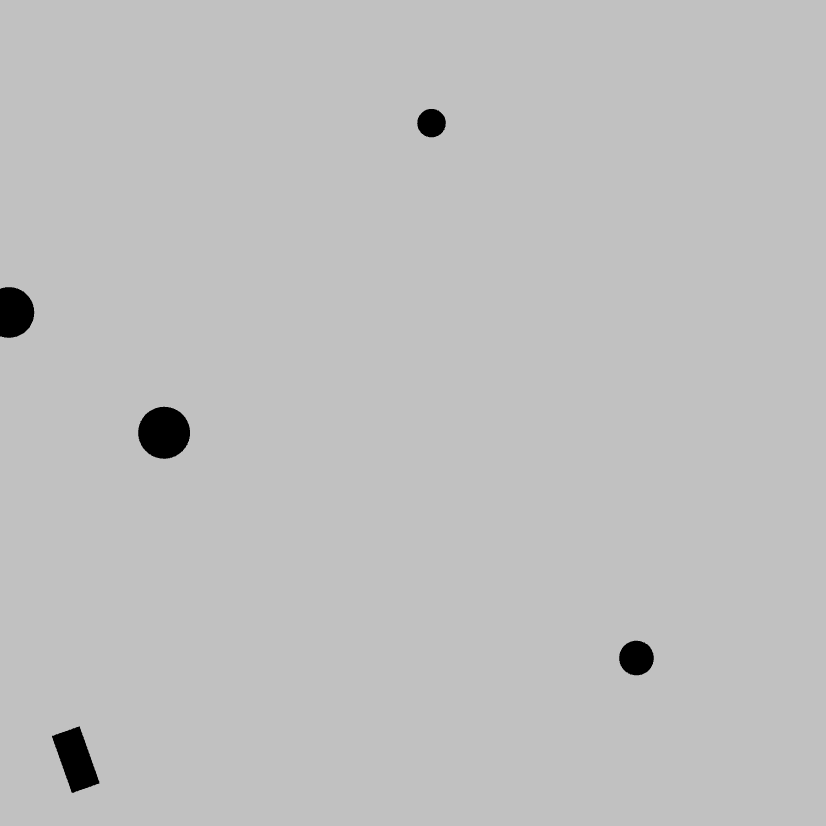
\includegraphics[width=1\linewidth]{graphics/test_model_05_5.png}
							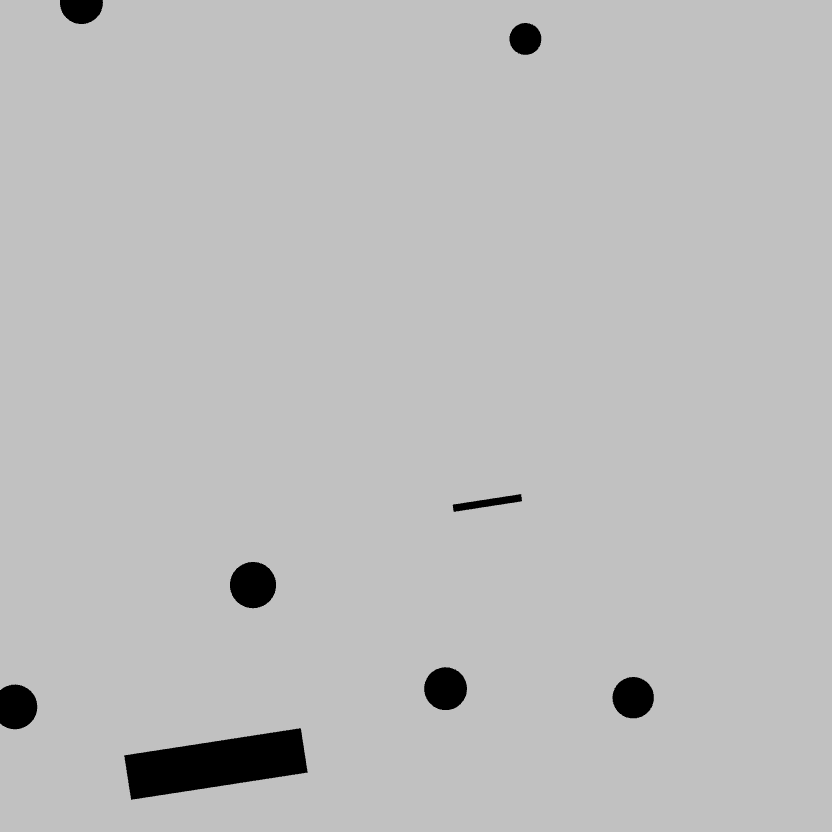
\includegraphics[width=1\linewidth]{graphics/test_model_08_5.png}
							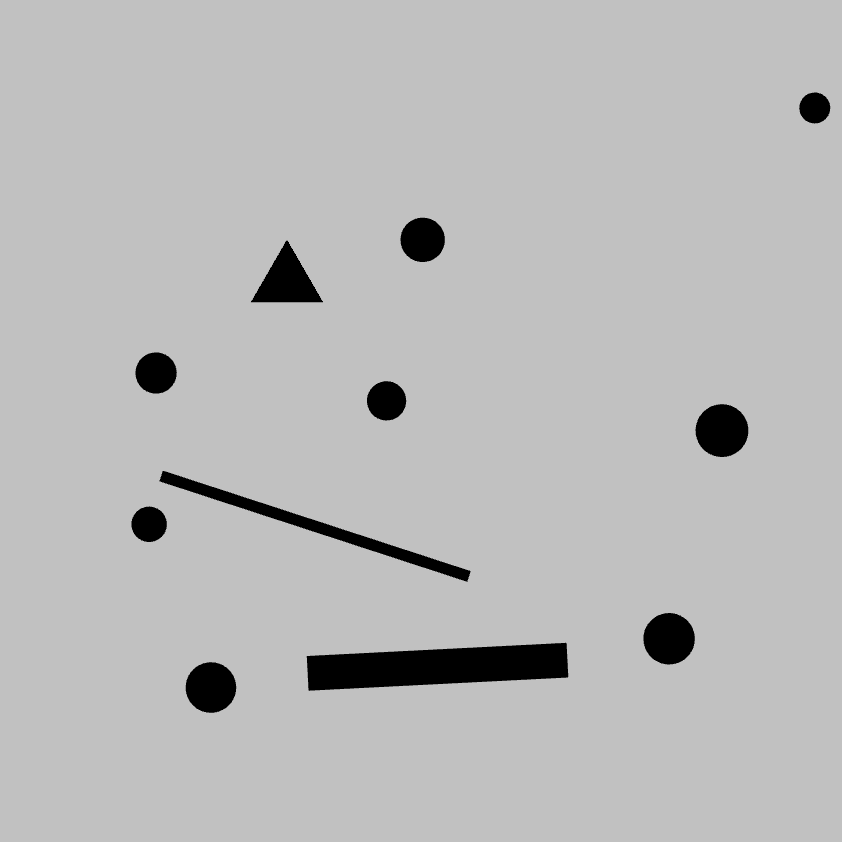
\includegraphics[width=1\linewidth]{graphics/test_model_11_5.png}
							
\includegraphics[width=1\linewidth]{graphics/test_model_15_5.png}
						\end{column}
						\begin{column}{0.05\textwidth}
						\end{column}
						\begin{column}{0.14\textwidth}
							\includegraphics[width=1\linewidth]{graphics/test_model_20_1.png}
							\includegraphics[width=1\linewidth]{graphics/test_model_30_1.png}
							\includegraphics[width=1\linewidth]{graphics/test_model_11_complex_1.png}
							\includegraphics[width=1\linewidth]{graphics/test_model_15_complex_1.png}
						\end{column}
					\end{columns}
				\end{figure}
			\end{frame}
		\subsection{Comparaison et analyse des résultats}
			\begin{frame}
				\frametitle{Expérimentations, validations et évaluations}
				\framesubtitle{Comparaison et analyse des résultats}
				\begin{figure}[H]
					\includegraphics[width=\linewidth]{graphics/investigation_polygonale-peinture_au_rouleau_ski_nordique-kappa_for_each_world_vs_investigation_polygonale-kappa_for_each_world.png}
				\end{figure}
			\end{frame}
			\begin{frame}
				\frametitle{Expérimentations, validations et évaluations}
				\framesubtitle{Comparaison et analyse des résultats}
				\begin{figure}[H]
					\includegraphics[width=\linewidth]{graphics/investigation_polygonale-peinture_au_rouleau_ski_nordique-time_for_each_world_vs_investigation_polygonale-time_for_each_world.png}
				\end{figure}
			\end{frame}
	\section{Bilan personnel}
		\begin{frame}
			\frametitle{Bilan personnel}
			\begin{itemize}
				\item Domaine de la recherche,
				\item Recherches bibliographiques,
				\item Robotique,
				\item Nouveaux outils techniques,
				\item Rédaction du rapport PFE.
			\end{itemize}
		\end{frame}
	\section{Conclusion et perspectives}
		\begin{frame}
			\frametitle{Conclusion et perspectives}
			\framesubtitle{Conclusion}
			\begin{itemize}
				\item Développement et évaluation de 3 stratégies de navigation pour la tomographie,
				\item État de l'art pauvre dans ce domaine
				\item Mise en place d'un environnement de simulation
				\item Mise en place d'un protocole d'évaluation avec métriques d'évaluation et scénarios de test
				\item Collecte de données et analyses statistiques
			\end{itemize}
		\end{frame}
		\begin{frame}
			\frametitle{Conclusion et perspectives}
			\framesubtitle{Perspectives}
			\begin{itemize}
				\item Gestion des collisions
				\item Simulation avec $k > 1$ équipes et $n > 2$ robots
				\item Déploiement sur des systèmes réels
			\end{itemize}
		\end{frame}
\end{document}